
\documentclass[a4paper,UKenglish,cleveref, autoref, thm-restate]{lipics-v2021}
%This is a template for producing LIPIcs articles.
%See lipics-v2021-authors-guidelines.pdf for further information.
%for A4 paper format use option "a4paper", for US-letter use option "letterpaper"
%for british hyphenation rules use option "UKenglish", for american hyphenation rules use option "USenglish"
%for section-numbered lemmas etc., use "numberwithinsect"
%for enabling cleveref support, use "cleveref"
%for enabling autoref support, use "autoref"
%for anonymousing the authors (e.g. for double-blind review), add "anonymous"
%for enabling thm-restate support, use "thm-restate"
%for enabling a two-column layout for the author/affilation part (only applicable for > 6 authors), use "authorcolumns"
%for producing a PDF according the PDF/A standard, add "pdfa"

%\pdfoutput=1 %uncomment to ensure pdflatex processing (mandatatory e.g. to submit to arXiv)
%\hideLIPIcs  %uncomment to remove references to LIPIcs series (logo, DOI, ...), e.g. when preparing a pre-final version to be uploaded to arXiv or another public repository

\usepackage{tikz-qtree}
\usetikzlibrary{positioning}
\usetikzlibrary{arrows.meta}
\usetikzlibrary{arrows,shapes,quotes}

%\graphicspath{{./graphics/}}%helpful if your graphic files are in another directory

\bibliographystyle{plainurl}% the mandatory bibstyle

\title{Embedding Intuitionistic into Classical Logic} %TODO Please add

%\titlerunning{Dummy short title} %TODO optional, please use if title is longer than one line

\author{Alexander {Pluska}}{Faculty of Mathematics, Universtät Wien, Austria}{e11941874@student.tuwien.ac.at}{https://orcid.org/my-orcid?orcid=0000-0002-7709-3335}{}%TODO mandatory, please use full name; only 1 author per \author macro; first two parameters are mandatory, other parameters can be empty. Please provide at least the name of the affiliation and the country. The full address is optional. Use additional curly braces to indicate the correct name splitting when the last name consists of multiple name parts.

\author{Florian Zuleger}{Institute of Logic and Computation, Technische Universität Wien, Austria}{florian.zuleger@tuwien.ac.at}{https://orcid.org/0000-0003-1468-8398}{}

\authorrunning{A. Pluska and F. Zuleger} %TODO mandatory. First: Use abbreviated first/middle names. Second (only in severe cases): Use first author plus 'et al.'

\Copyright{Alexander Pluska and Florian Zuleger} %TODO mandatory, please use full first names. LIPIcs license is "CC-BY";  http://creativecommons.org/licenses/by/3.0/

\ccsdesc[100]{\textcolor{red}{Theory of Computation Logic Constructive Mathematics}} %TODO mandatory: Please choose ACM 2012 classifications from https://dl.acm.org/ccs/ccs_flat.cfm

\keywords{Intuitionistic Logic, Automated Reasoning, Propositional Logic, First-order Logic, QBF} %TODO mandatory; please add comma-separated list of keywords

\category{} %optional, e.g. invited paper

\relatedversion{} %optional, e.g. full version hosted on arXiv, HAL, or other respository/website
%\relatedversiondetails[linktext={opt. text shown instead of the URL}, cite=DBLP:books/mk/GrayR93]{Classification (e.g. Full Version, Extended Version, Previous Version}{URL to related version} %linktext and cite are optional

%\supplement{}%optional, e.g. related research data, source code, ... hosted on a repository like zenodo, figshare, GitHub, ...
%\supplementdetails[linktext={opt. text shown instead of the URL}, cite=DBLP:books/mk/GrayR93, subcategory={Description, Subcategory}, swhid={Software Heritage Identifier}]{General Classification (e.g. Software, Dataset, Model, ...)}{URL to related version} %linktext, cite, and subcategory are optional

%\funding{(Optional) general funding statement \dots}%optional, to capture a funding statement, which applies to all authors. Please enter author specific funding statements as fifth argument of the \author macro.


%\nolinenumbers %uncomment to disable line numbering



%Editor-only macros:: begin (do not touch as author)%%%%%%%%%%%%%%%%%%%%%%%%%%%%%%%%%%
\EventEditors{John Q. Open and Joan R. Access}
\EventNoEds{2}
\EventLongTitle{42nd Conference on Very Important Topics (CVIT 2016)}
\EventShortTitle{CVIT 2016}
\EventAcronym{CVIT}
\EventYear{2016}
\EventDate{December 24--27, 2016}
\EventLocation{Little Whinging, United Kingdom}
\EventLogo{}
\SeriesVolume{42}
\ArticleNo{23}
%%%%%%%%%%%%%%%%%%%%%%%%%%%%%%%%%%%%%%%%%%%%%%%%%%%%%%

\begin{document}

\maketitle

%TODO mandatory: add short abstract of the document
\begin{abstract}
The famous double negation translation~\cite{glivenko1929quelques, godel1933intuitionistischen} establishes an embedding from classical into intuitionistic logic. Curiously the reverse direction has not been covered in literature. We present an effective embedding from intuitionistic into classical logic, both in the propositional and first-order case, as well as an effective embedding of intuitionistic propositional logic into quantified boolean formulas.
Furthermore, in the propositional case we establish a parameter that bounds the proof complexity of intuitionistic formulas. As part of our construction, we also present a Tseytin-like translation that preserves intuitionistic validity and reduces formulas to a normal form. 

%The key notion used in the proofs is the existence of counter-models - an analogon to the satisfiability of the negation in classical logic, which is not equivalent to invalidity in the intuitionistic case.  We hope that this will allow leveraging the tremendous recent progress in automated reasoning in classical logic for checking intuitionistic validity, for which there has not been much progress in recent decades.


We hope that our embeddings of classical into intuitionistic logic will allow leveraging the tremendous progress in automated reasoning in classical logic for checking intuitionistic validity, for which there has not been much progress in recent decades. Crucially, our constructions support the transfer of counter-models to validity, which is important to model checking applications, where the output of counter-examples is an appreciated feature.
\end{abstract}

\section{Introduction}

Constructive mathematics refers to a flavour of mathematics in which existence of an object can only be established by explicit construction, as opposed to classical mathematics where existence can be shown implicitly, e.g. by assuming non-existence and deriving a contradiction. Besides the philosophical issues that one may take with classical mathematics, most prominently advocated by Brouwer~\cite{brouwer1907over} and Bishop~\cite{bishop1967foundations}, there is a particular motivation when looking from the position of computer science in that intuitionistic proofs correspond directly to computer programs, which is expressed in the Curry-Howard-Isomorphism~\cite{howard1980formulae}. The formalism usually associated with constructive mathematics is intuitionistic logic, which essentially differentiates itself from classical logic by the facts that the law of excluded middle $A\vee\neg A$ and double negation shift $\forall x\neg\neg P(x)\to\neg\neg\forall xP(x)$ are not valid.

However comparing benchmarks for classical and intuitionistic automated theorem proving, e.g. TPTP~\cite{casc} and ILTP~\cite{iltp}, we see that classical provers currently have a far better success rate. Furthermore all the most popular and used first-order provers~\cite{kovacs2013first, schulz2002brainiac, korovin2008iprover} utilize classical logic. This difference can be partially explained by fundamental differences between the logics. First of all in the propositional case determining intuitionistic validity is \verb+PSPACE+-complete~\cite{statman1979intuitionistic} whereas the analogous decision problem for classical logic is only \verb+coNP+-complete~\cite{cook1971complexity}. A further advantage of classical logic is the existence of calculi that are particularly suitable for automation like superposition~\cite{bachmair2001resolution} which rely on the existence of convenient normal forms such as CNF and the duality between validity and satisfiability, i.e. to show validity they show unsatisfiability of the negation. While some kind of normal form would of course obtainable in the intuitionistic case, crucially the duality does not hold, e.g. $\neg(A\vee \neg A)$ is not satisfiable while $A\vee\neg A$ is not a theorem. Therefore most dedicated intuitionistic theorem provers~\cite{mclaughlin2009efficient, tammet1996resolution} use the naive inverse method, i.e. directly constructing a cut-free proof, enhanced by search strategies such as focussing and polarization. This strategy generally leads to a much more complex search and is difficult to implement efficiently. Finally in contrast to intuitionistic provers a tremendous amount of work has been put into optimizing provers for classical logic, this is particularly true for the propositional case, i.e. SAT-solvers.

With this work we want to open the path for leveraging the progress that has been made in classical theorem proving for intuitionistic logic. To that end we give an embedding from intuitionistic logic into classical logic. That is we give an effective procedure that gives for each formula $\varphi$ we a modified formula $\varphi^\#$ such that $\varphi$ is intuitionistically valid if and only if $\varphi^\#$ is classically valid. Interestingly the reverse direction, the famous double negation translation, is a long established translation that goes back to Glivenko~\cite{glivenko1929quelques} in the propositional case and G\"odel~\cite{godel1933intuitionistischen} and Gentzen~\cite{gentzen1936widerspruchsfreiheit} in the first-order case. In the propositional case it is particularly simple: $\varphi$ is classically valid if and only if $\neg\neg\varphi$ is intuitionistically valid. Intuitively the translation collapses for each subformula $\psi$ the truth values of $\psi$ and $\neg\neg\psi$, which are classically but not intuitionistically equivalent. This gives us a first idea why the reverse direction is perhaps more difficult: We need to expand the truth values of $\psi$ and $\neg\neg\psi$, i.e. if they both occur in $\varphi$ we must have a way to (classically) assign different truth values to their respective counterparts in $\varphi^\#$. In particular this necessitates the introduction of new propositional variables, which already marks a big difference to the double negation translation.

In addition to the translation of formulas we give an effective translation of counter-models, i.e. for each intuitionistic counter-model for $\varphi$ we give a classical counter-model for $\varphi^\#$ and vice versa. In fact the existence of counter-models is a key notion. For classical logic it just corresponds to the satisfiability of the negation. However for intuitionistic logic it forms a proper dual to validity, while satisfiability of the negation is not necessary for invalidity and would therefore not form a proper dual. Transforming and reducing counter-models is what ultimately enables our translation.

Finally we should mention that approaches to obtain constructive content from classical proofs exist in literature, however they are insufficient in our view. The first is simply to examine under which circumstances classical validity entails intuitionistic validity and therefore constructiveness. Most famously this holds for $\Pi_2$-formulas in Peano Arithmetic~\cite{friedman1978classically}. There are also other circumstances under which this entailment holds~\cite{schwichtenberg}, however this approach cannot encapsulate the general case. Another popular approach is to equip classical proofs with operational semantics~\cite{Control1, Parigot1}. In this case we necessarily lose realizability at least of $\exists$ and $\vee$, which - one could argue - is why we want a program in the first place.

We suggest a new approach for obtaining a constructive proof using a classical prover:
\begin{itemize}
	\item Performing our translation on the input formula $\varphi$ to obtain $\varphi^\#$.
	\item Checking the classical validity of $\varphi^\#$ with the prover resulting in a proof or counter-model.
	\item Translating the proof/counter-model of $\varphi^\#$ to a (intuitionistic) proof/counter-model of $\varphi$.
\end{itemize}



\section{Overview}

We shall now give an overview of the main results and highlight the key arguments. Recall that our goal is to give an effective translation procedure that, for a given formula $\varphi$, yields a formula $\varphi^\#$ such that $\varphi$ is intuitionistically valid if and only if $\varphi^\#$ is classically valid. We start with the predicate case. The key arguments are the same as in the first-order case while it is technically simpler and less cluttered and therefore more clear.

Before performing the main transformation we propose a preprocessing to a simpler form. A popular pre-processing step in classical automated reasoning is the Tseytin transformation~\cite{tseitin1983complexity}. It gives an equisatisfiable sentence in conjunctive normal form. Eliminating all implications is not possible in intuitionistic logic since $A\to B$ is not equivalent to $\neg A\vee B$. Still we propose a similar transformation. A nice feature will be that the non-classical content will be encapsulated in formulas of type $(A\to B)\to C$, i.e. if there are no such formulas in the transformed formula then the classical validity of the original formula immediately implies intuitionistic validity.

\begin{theorem}
	For every propositional formula $\varphi$ there exists an effective procedure that yields an atom $P$ and a set of $\mathcal S$ of formulas  of one of the forms
	$$A\to (B\wedge C), (A\wedge B)\to C, A\to (B\vee C), (A\vee B)\to C, (A\to B)\to C$$for atomic $A, B, C$ such that $\varphi$ is intuitionistically valid if and only if $\bigwedge\mathcal S\to P$ is intuitionistically valid. The size of $\mathcal S$ and time complexity of the transformation are linear in the input size.
\end{theorem}

The main transformation then proceeds in three steps.

First we encode as a first-order sentence that the considered formula holds in every Kripke frame. Since Kripke frames for propositional logic over a fixed alphabet of propostional variables form a first-order theory this is rather straightforward.

Next we eliminate some quantifiers via Herbrandization. The only quantifiers eliminated occur in formulas derived from formulas of type $(A\to B)\to C$.

This leaves us with a formula with only weak $\forall$-quantifiers. We can then argue that if there is a counter-model for the resulting formula then there is a counter-model with a certain Kripke frame completely determined by the number of formulas of type $(A\to B)\to C$. This allows us to eliminate the remaining quantifiers by simply enumerating the worlds in that Kripke model.

All in all this leaves us with the following:

\begin{theorem}
	Let $\mathcal S$ be as above. Let $\mathcal F_\to\subseteq\mathcal S$ denote formulas $\psi$ of the form $(A_\psi\to B_\psi)\to C_\psi$ and $\Lambda$ denote the set of sequences without repetition over $\mathcal F_\to$. For each atom $A$ and $k\in\Lambda$ consider a new atom $A^k$. Obtain $\mathcal S^\#$ by including formulas as follows
	\begin{itemize}
		\item $A^k\to A^{k\psi}$ for each atom $A$ occurring in $\mathcal S$, $k\in\Lambda$ and $\psi\in\mathcal F_\to$ not occurring in $k$.
		\item $A^k\to (B^k\circ C^k)$ for each $\circ\in\{\wedge,\vee\}$, $A\to (B\circ C)\in\mathcal S$, $k\in\Lambda$.
		\item $(A^k\circ B^k)\to C^k$ for each $\circ\in\{\wedge,\vee\}$, $A\to (B\circ C)\in\mathcal S$, $k\in\Lambda$.
		\item $(A^{k\psi}\to B^{k\psi})\to C^k$ for $\psi = (A\to B)\to C\in\mathcal S$, $k\in\Lambda$ if $\psi$ does not occurr in $k$.
	\end{itemize}
	Then $\bigwedge S\to P$ is intuitionistically valid iff $\bigwedge S^\#\to P^\epsilon$ is classically valid, where $\epsilon$ denotes the empty sequence. The size of $\mathcal S^\#$ is in $\mathcal O(|\mathcal S|\cdot2^{|\mathcal F_\to|\cdot\log(|\mathcal F_\to|)})$. Futhermore there is an effective procedure for translating counter-models between the sentences.
\end{theorem}

Examining the proof of the above theorem we will be able to notice that due to its tree form the constructed Kripke frame lends itself as an interpretation for a certain quantified boolean formula. We can show that this QBF is satisfiable if and only if there exists a counter-model for our original formula.

\begin{theorem}
	Let $\mathcal S$ be as above. There is an effective procedure that produces a QBF $\varphi^Q$ of size $\mathcal O(|\mathcal S|\cdot|\mathcal F_\to| + |\mathcal F_\to|^3)$ with $2\cdot |\mathcal F_\to|-1$ quantifier alternations such that $\varphi$ is intuitionistically valid if and only if $\varphi^Q$ is not satisfiable. Fixing $N\in\mathbb N$ deciding intuitionistic validity for formulas $\bigwedge \mathcal S\to P$ where $\mathcal S$ is as above and $|\mathcal F_\to| = N$ is therefore in $\Sigma_{2N-1}$.
\end{theorem}

We then move to the first-order case. Here things are a bit more involved but the underlying approach is the same. First we again perform a Tseytin-like transformation. Here the non-classical content is encapsulated by formulas of type $(A\to B)\to C$ and $\forall xA\to B$.

\begin{theorem}
	For every predicate formula $\varphi$ there exists an effective procedure that yields an atom $P$ and a set $\mathcal S$ of formulas of the forms
	$$\forall \vec z(A(\vec a)\to (B(\vec b)\wedge C(\vec c))), \forall \vec z((A(\vec a)\wedge B(\vec b))\to C(\vec c)),$$$$\forall \vec z(A(\vec a)\to (B(\vec b)\vee C(\vec c))),
	\forall \vec z((A(\vec a)\vee B(\vec b))\to C(\vec c)),$$$$ \forall \vec z((A(\vec a)\to B(\vec b))\to C(\vec c)),\forall \vec z(\forall xA(\vec a)\to B(\vec b)),$$$$ \forall \vec z(A(\vec a)\to\forall xB(b)), \forall \vec z(\exists xA(\vec a)\to B(\vec b)), \forall \vec z(A(\vec a)\to\exists xB(b))$$for atomic $A, B, C$ and vectors of variables $\vec z, \vec a, \vec b, \vec c$ such that $\varphi$ is intuitionistically valid if and only if $\bigwedge\mathcal S\to P$ is intuitionistically valid. The size of $\mathcal S$ and time complexity of the transformation are linear in the input size.
\end{theorem}

We then proceed quite similarly to the propositional case. Note however that one difficulty arises from the fact that our (classical) domain will now contain on the one hand worlds in the Kripke frame but on the other hand also proper domain elements. We resolve this apparent conflict by introducing a special binary predicate $E$, inspired by~\cite{iemhoff2010eskolemization}, encoding which domain elements exists at which world. In particular $E(x, u)$ entails that $x$ represents a domain element and $u$ a world.

The Herbrandization is completely analogous the the propositional case.

The real difference arises in the final step: While we can also establish a universal Kripke Frame that is parametrized only by the formulas of type $(A\to B)\to C$ and $\forall xA\to B$, it is possibly countably infinite. This is not surprising since certain intuitionistically invalid formulas like the double negation shift $\forall x\neg\neg A(x)\to \neg\neg\forall x A(x)$ don't have finite counter-models. Therefore we are not able to eliminate the weak $\forall$-quantifiers associated with the Kripke semantics. However since we started in first-order logic to begin with this is perhaps not a big deal.

We end up with the following translation:

\begin{theorem}\label{fullFOtranslation}
	Let $\mathcal S$ be as above and $\mathcal F_\to\subseteq\mathcal S$ contain formulas of the form $\forall \vec t((A(\vec z_A)\to B(\vec z_B))\to C(\vec z_C))$ and $\mathcal F_\forall\subseteq\mathcal S$ the formulas of the form $\forall \vec z(\forall xA(\vec z_A)\to B(\vec z_B))$. Let $\mathcal F = \mathcal F_\to\cup\mathcal F_\forall$. For every $n$-ary atomic relation $R$ define a new $n+1$-ary relation $R^\#$. For every $\psi\in\mathcal F$ define a new function symbol $f_\psi$. Consider a new binary relation symbol $E$ and define $\vec E(\vec x, u) := \bigwedge\{E(x, u)\:|\:x\in\vec x\}$. Obtain $\mathcal S^\#$ by including formulas as follows:
	\begin{itemize}
		\item $\forall \vec z\forall u(\vec E(\vec z, u)\to (A^\#(\vec a, u)\to (B^\#(\vec b, u)\circ C^\#(\vec c, u))))$\\for each $\circ\in\{\wedge, \vee\}, \psi = \forall \vec z(A(\vec a)\to (B(\vec b)\circ C(\vec c)))\in\mathcal S$
		\item $\forall \vec z\forall u(\vec E(\vec z, u)\to (A^\#(\vec a, u)\circ B^\#(\vec b, u))\to C^\#(\vec c, u))$\\for each $\circ\in\{\wedge, \vee\}, \psi = \forall \vec z((A(\vec a)\circ B(\vec b))\to C(\vec c))\in\mathcal S$
		\item $\forall \vec z\forall u(\vec E(\vec z, u)\to(A^\#(\vec a, f(\vec z, u))\to B^\#(\vec b, f(\vec z, u)))\to C^\#(\vec c, u))$ for each $\psi = \forall \vec z((A(\vec a)\to B(\vec b))\to C(\vec c))\in\mathcal S$
		\item  $\forall \vec z\forall u(\vec E(\vec z, u)\to \forall x(E(x, f(\vec z, u))\to A^\#(\vec a, f(\vec z, u)))\to B^\#(\vec b, u))$\\for each $\forall \vec z(\forall xA(\vec a)\to B(\vec t_B))\in\mathcal S$.
		\item $\forall \vec z\forall u(\vec E(\vec z, u)\to A^\#(\vec a, u)\to \forall x(E(x, u)\to B^\#(\vec b, u)))$\\for each $\forall \vec t(A(\vec a)\to \forall xB(\vec b))\in\mathcal S$.
		\item $\forall \vec z\forall u(\vec E(\vec z, u)\to \exists x(E(x, u)\wedge A^\#(\vec z, u))\to B^\#(\vec b))$\\for each $\forall \vec z(\exists xA(\vec a)\to B(\vec b))\in\mathcal S$
		\item $\forall \vec z\forall u(\vec E(\vec z, u)\to A^\#(\vec b)\to \exists x(E(x, u)\wedge B^\#(\vec b, u)))$\\for each $\forall \vec z(A(\vec a)\to \exists xB(\vec b))\in\mathcal S$
	\end{itemize}
	Then $\bigwedge S\to P$ is intuitionistically iff $\exists xE(x, s)\to K\to \bigwedge\mathcal S^\#\to P^\#(s)$ is classically valid, where $s$ is a new constant symbol, $\Sigma$ is the original signature and
	\begin{align*}
		K := &\:\bigwedge\{\forall x\forall u((E(x, u)\to E(x, f_\psi(u)))\:|\:\psi\in\mathcal F\}\wedge\\
		&\:\forall u\left(\exists xE(x, u)\to \bigwedge\{\forall\vec z(\vec E(\vec z, u)\to E(f(\vec z), u))\:|\:\text{$f$ is a function symbol in $\Sigma$}\}\right)\wedge\\
		&\:\bigwedge\{\forall\vec z_1\forall \vec z_2\forall u(A^\#(\vec z_1, u)\to A^\#(\vec z_1, f_\psi(\vec z_2, u)))\:|\:\text{$\psi\in\mathcal F$, $A$ is a relation symbol in $\Sigma$}\}
	\end{align*}
	The size of the obtained formula is linear in the input. However a $|\mathcal F| + 1$ new function symbols and the new binary predicate $E$ were introduced and each $n$-ary relation symbol has been extended to a $n+1$-ary relation symbol.
\end{theorem}

These results provide an effective framework for using classical provers to check intuitionistic validity. First experiments with the Vampire theorem prover show promise.


\section{Preliminaries}

Before proceeding towards the results let us quickly fix our notation and recapitulate the semantics for intuitionistic logic.

\subsection{Propositional Semantics}

\begin{definition}
	A \textbf{valuation} $v$ is a function that assigns to each propositional variable $A$ a \textbf{truth value} $v(A)\in\{0, 1\}$. We extend $v$ to a function $v^*$ on formulas:
	\begin{itemize}
		\item $v^*(\bot) = 0$
		\item $v^*(A) = v(A)$ for each propositional variable $A$.
		\item $v^*(\varphi\wedge\psi) = \min(v^*(\varphi), v^*(\psi))$
		\item $v^*(\varphi\vee\psi) = \max(v^*(\varphi), v^*(\psi))$
		\item $v^*(\varphi\to \psi) = \max(1 - v^*(\varphi), v^*(\psi))$
	\end{itemize}
	$v$ is a \textbf{model} for $\varphi$ if $v(\varphi) = 1$. We denote the set of valid formulas with CPC.
\end{definition}

One notable property of classical logic is that a formula $\varphi$ is valid if and only if its negation, i.e. $\neg\varphi$ is not satisfiable. The same does not hold true for intuitionistic logic as we shall see.

\begin{definition}
	A \textbf{Kripke structure} $\mathcal K = (W, (v_w)_{w\in W})$ consists of a partially ordered set $W$ of nodes an a family of valuations $(v_w)_{w\in W}$ such that for $u\leq w$ we have $v_u(A)\leq v_u(A)$ for every propositional variable $A$, this is called the \textbf{persistency condition}. We extend the valuations $v_u$ slightly differently to $v_u^\#$ than before, i.e. have
	\begin{itemize}
		\item $v_u^\#(\bot) = 0$
		\item $v_u^\#(\varphi) = v_u(A)$ if $\varphi$ is atomic.
		\item $v_u^\#(\varphi\wedge\psi) = \min(v_u^\#(\varphi), v_u^\#(\psi))$
		\item $v_u^\#(\varphi\vee\psi) = \max(v_u^\#(\varphi), v_u^\#(\psi))$
		\item $v_u^\#(\varphi\to \psi) = \min\{\max(1 - v_w^\#(\varphi), v_w^\#(\psi))\:|\:w\geq u\}$
	\end{itemize}
	That is $v_u^\#(\varphi\to \psi) = 1$ if at every world $w\geq u$ we have $v_w^\#(\varphi) = 0$ or $v_w^\#(\psi) = 1$. We say that $\varphi$ is satisfied at a node $u$ if $v_u^\#(\varphi) = 1$ and write $u\models\varphi$. If a formula is satisfied at every node then $\mathcal K$ is a \textbf{model} for $\varphi$. We denote the set of valid formulas with IPC.
\end{definition}
There are many classical tautologies which are not intuitionistically valid
\begin{example}\label{LEMcounterexample}
	Consider the famous law of excluded middle $A\vee\neg A$. Recall that $\neg A := A\to \bot$. As a counter-model consider a Kripke structure with two nodes $u\leq w$ and $v_u(A) = 0, v_w(A) = 1$. Then $u\not\models A$ and $u\not\models \neg A$, i.e. $u\not\models A\vee\neg A$. 
\end{example}
In classical logic a proven strategy for showing that a formula valid is to consider its negation and show that it is not satisfiable. This is insufficient for intuitionistic logic, e.g. $A\vee\neg A$ is not a intuitionistic tautology but its negation is not satisfiable either.



\subsection{Predicate Semantics}

We now give account of the more involved semantics of first-order logic

\begin{definition}
	Let $\Sigma$ be a signature. A $\Sigma$-structure $\mathcal{M}$ consists of a non-empty set $M$, the domain of $\mathcal{M}$, and a function $I$ that assigns
	\begin{itemize}
		\item to each $n$-ary function symbol $f$ a $n$-ary function $f^I: M^n\to M$.
		\item to each $n$-ary relation symbol $R$ a $n$-ary relation $R^I\subseteq M^n$.
	\end{itemize}
	A variable assignment $v$ is a function that assigns to each free variable an element $m\in M$. For each free variable $a$ and $m\in M$ we define $$v[m/a](b) = \begin{cases}
		m&\text{if $b=a$}\\
		v(b)&\text{otherwise}
	\end{cases}$$
	Then terms are interpreted as follows:
	\begin{itemize}
		\item $a^{I, v} = v(a)$ for each free variable $a$.
		\item $f(t_1,\dots,t_n)^{I, v} = f^I(t_1^{I, v},\dots, t_n^{I, v})$.
	\end{itemize}
	We define a model relation between pairs $\mathcal M, v$ and formulas $\varphi$ as follows
	\begin{itemize}
		\item $\mathcal M, v\not\models\bot$.
		\item $\mathcal M, v\models R(t_1,\dots,t_n)$ iff $(t_1^{I, v},\dots,t_n^{I, v})\in R^I$.
		\item $\mathcal M, v\models s = t$ iff $s^{I, v} = t^{I, v}$.
		\item $\mathcal M, v\models \varphi\wedge \psi$ iff $\mathcal M, v\models\varphi$ and $\mathcal M, v\models\psi$.
		\item $\mathcal M, v\models \varphi\vee\psi$ iff $\mathcal M, v\models\varphi$ or $\mathcal M, v\models\psi$.
		\item $\mathcal M, v\models \varphi\to\psi$ iff $\mathcal M, v\not\models\varphi$ or $\mathcal M, v\models\psi$.
		\item $\mathcal M, v\models\exists x\varphi$ iff there exists $m\in M$ such that $\mathcal M, v[m/a]\models\varphi[a/x]$ where a is a free variable that does not occur in $\varphi$.
		\item $\mathcal M, v\models\forall x\varphi$ iff for all $m\in M$ we have $\mathcal M, v[m/a]\models\varphi[a/x]$ where a is a free variable that does not occur in $\varphi$.
	\end{itemize}
	$\mathcal{M}$ satisfies $\varphi$ if $\mathcal M, v\models\varphi$ for every $v$. We denote the set of valid formulas with CQC.
\end{definition}

\begin{definition}
	A $\Sigma$-\textit{Kripke structure} $\mathcal{K}$ is a partially ordered set $W$ and a family of $\Sigma$-structures $(\mathcal{M}_w)_{w\in W}$ such that for $u\leq w$
	\begin{itemize}
		\item $M_u\subseteq M_w$.
		\item $f^{I_w}|_{M_u} = f^{I_u}$.\footnote{Here $f|_M$ denotes the restriction of $f$ to $M$}
		\item $R^{I_w}|_{M_u} = R^{I_u}$.
	\end{itemize}
	Then we define a model relation between worlds $u\in W$ and variable assignments $v$ (targeting $M_u$) and formulas $\varphi$ as follows:
	\begin{itemize}
		\item $u, v\not\models\bot$
		\item $u, v\models R(t_1,\dots,t_n)$ iff $(t_1^{I_u, v},\dots,t_n^{I_u, v})\in R^{I_u}$.
		\item $u, v\models s = t$ iff $s^{I_u, v} = t^{I_u, v}$.
		\item $u, v\models \varphi\wedge \psi$ iff $u, v\models\varphi$ and $u, v\models\psi$.
		\item $u, v\models \varphi\vee\psi$ iff $u, v\models\varphi$ or $u, v\models\psi$.
		\item $u, v\models \varphi\to\psi$ iff for every $w\geq u$ we have $w, v\not\models\varphi$ or $w, v\models\psi$.
		\item $u, v\models\exists x\varphi$ iff there exists $m\in M_u$ such that $u, v[m/a]\models\varphi[a/x]$ where a is a free variable that does not occur in $\varphi$.
		\item $u, v\models\forall x\varphi$ iff for every $w\geq u$ and $m\in M_w$ we have $w, v[m/a]\models\varphi[a/x]$ where a is a free variable that does not occur in $\varphi$.
	\end{itemize}
	$\mathcal{K}$ satisfies $\varphi$ if $u, v\models\varphi$ holds for every world $u$ and variable assignment $v$. We denote the set of valid formulas with IQC.
\end{definition}
In addition to the propositional tautologies there are now sentences involving quantifiers which are classically valid but not intuitionistically.
Consider for instance the classical tautology $\varphi$ $$\neg\forall x A(x)\to \exists x \neg A(x)$$Analogous remarks with regard to validity and satisfiability hold as in the propositional case.

\subsection{Skolemization and Herbrandization}
An important step in the embedding will be the elimination of quantifiers via Herbrandization. In this process we introduce free variables and also additional function symbols to the signature. Whenever we speak of a new free variable what is meant is a free variable that does not occur in any of the considered formulas. Whenever a new function symbol is introduced we implicitly extend the signature by some not previously contained symbol.

\begin{definition}
	For formulas $\varphi$ we define the Skolemization $\varphi^S_Z$ and Herbrandization $\varphi^H_Z$ with respect to $Z$ by simultaneous induction as follows:
	\begin{itemize}
		\item $A^S_T = A^H_Z = A$ for each atomic $A$.
		\item $(\varphi\circ\psi)^X_Z = \varphi^X_Z\circ\psi^X_Z$ for $\circ\in\{\wedge, \vee\}$, $X\in\{S, H\}$.
		\item $(\varphi\to\psi)^S_Z = \varphi^H_Z\to \psi^S_Z$\\$(\varphi\to\psi)^H_Z = \varphi^S_Z\to\psi^H_Z$.
		\item $(\forall x\varphi)^S_Z = \forall x(\varphi[a/x]^S_{T\cup\{a\}}[x/a])$ where $a$ is a new free variable\\$(\forall x\varphi)^H_Z = \varphi[s(z_1,\dots,z_n)/x]^H_Z$ where $s$ is a new function, $\{z_1\dots z_n\} = Z$.
		\item $(\exists x\varphi)^S_Z = \varphi[s(z_1,\dots,z_n)/x]^S_Z$ where $s$ is a new function, $\{z_1\dots z_n\} = Z$\\$(\exists x\varphi)^H_Z = \exists x(\varphi[a/x]^H_{Z\cup\{a\}}[x/a])$ where $a$ is a new free variable.
	\end{itemize}
	Let $\varphi^S = (\exists x_1\dots\exists x_n \varphi[x_1/a_1\dots x_n/a_n])^S_\emptyset$ and $\varphi^H = (\forall x_1\dots\forall x_n \varphi[x_1/a_1\dots x_n/a_n])^H_\emptyset$ where $a_1,\dots,a_n$ are the free variables occurring in $\varphi$.
\end{definition}

\begin{theorem}For every formula $\varphi$
	\begin{itemize}
		\item $\varphi$ and $\varphi^S$ are classically equisatisfiable.
		\item $\varphi$ and $\varphi^H$ are classically equivalid.
	\end{itemize}
\end{theorem}

which follows from Lemmata~\ref{ap1} and~\ref{ap2} in the appendix. We are now ready to present our embedding of intuitionistic into classical logic.



\section{IPC to CQC}

The most obvious approach to embedding intuitionistic into classical logic is to express intuitionistic semantics, i.e. Kripke frames, as a first order theory. For every propositional variable $A$ consider a unary predicate $A$ of the same name where $A(u)$ expresses that $A$ is true at some world $u$. We can then naively encode formulas as follows:

\begin{definition}
	Let $\varphi$ be a propositional formula. Define $\varphi^{u}$ inductively as follows:
	\begin{itemize}
		\item $A^{u} = A(u)$ for every propositional variable $A$.
		\item $\bot^u = \bot$.
		\item $(\varphi\circ\psi)^u = \varphi^u\circ\psi^u$ for $\circ\in\{\wedge, \vee\}$.
		\item $(\varphi\to \psi)^u = \forall w(u\preceq w\to\varphi^{w}\to\psi^{w})$ where $w$ is some new variable.
	\end{itemize}
	Let $K(\varphi)$ encode the Kripke semantics, i.e.
	$$K(\varphi) = \text{\normalfont PartialOrder}(\preceq)\wedge\forall u\forall w(u\preceq w\to \text{\normalfont Persistent}(u, w))$$
	with e.g.
	\begin{align*}
		\text{\normalfont PartialOrder}(\preceq) =&\:\forall u(u\preceq u)\wedge\forall u\forall w(u\preceq w\to w\preceq u\to u = w)\wedge\\&\:\forall u\forall v\forall w(u\preceq v\to v\preceq w\to u\preceq w)\\
		\text{\normalfont Persistent}(u, w)=&\:\bigwedge \{A(u)\to A(w))\:|\: \text{ $A$ is a propositional variable that occurs in $\varphi$}\}
	\end{align*}
	Then define
	$$\varphi^{C} = K(\varphi)\to \varphi^{u}$$
	where $u$ is some free variable.
\end{definition}

All that we have done is model Kripke frames with a finite number of propositional variables as a first-order theory and by definition we have

\begin{lemma}
	$\varphi$ is intuitionistically valid iff $\varphi^C$ is classically valid.
\end{lemma}

\begin{example}
	Consider the law of excluded middle $$\varphi = (A\to \bot)\vee A$$ which is not intuitionistically valid. Then
	\begin{align*}
		\varphi^{C} &= K(\varphi)\to ((A\to \bot)\vee A)^u\\
		&= K(\varphi)\to (A\to \bot)^u\vee A^u\\
		&= K(\varphi)\to (\forall u'( u\preceq u' \to A^{u'}\to \bot^{u'})\vee A(u))\\
		&= K(\varphi)\to (\forall u' (u\preceq u' \to A(u')\to \bot)\vee A(u))
	\end{align*}
	and indeed $\varphi^{C}$ admits a counter model with domain $\{u, u'\}$ where $u \preceq u'$, $A(u) = 0, A(u') = 1$.
\end{example}


\section{Equivalid normalization}

Of course transforming a propositional formula into a predicate formula is somewhat unsatisfying. As a first step we want to apply Herbrandization. Now trying to apply it to arbitrary formulas presents us with quite a leap in complexity, leading to nested expressions that will make arguments more complicated. We therefore propose a Tseytin-like transformation that produces a formula of a more manageable syntactic form. A similar translation was proposed in~\cite{statman1979intuitionistic}.

\begin{definition}
	Let $\varphi$ be some formula. For each sub(semi)formula $\psi$ of $\varphi$ consider some new $n$-ary relation symbol $P_\psi$ where $n$ is the number of variables occurring in $\psi$ that is not quantified within $\psi$. We denote those variables with $\vec z_\psi$ in some arbitrary but fixed order. We inductively define clause sets $\mathcal S^+(\varphi)$ and $\mathcal S^-(\varphi)$ as follows:
	\begin{itemize}
		\item For every atomic formula $A$\\$\mathcal S^+(A) = \{P_A(\vec z_A)\to A\}$\\$\mathcal S^-(A) = \{A\to P_A(\vec z_A)\}$
		\item For every conjunction or disjunction $\varphi\circ\psi$ with $\circ\in\{\wedge,\vee\}$\\$\mathcal S^+(\varphi\circ\psi) = \{P_{\varphi\circ\psi}(\vec z_{\varphi\circ\psi})\to P_{\varphi}(\vec z_\varphi)\circ P_{\psi}(\vec z_\psi)\}\cup \mathcal S^+(\varphi)\cup \mathcal S^+(\psi)$\\$\mathcal S^-(\varphi\circ\psi) =\{P_{\varphi}(\vec z_\varphi)\circ P_{\psi}(\vec z_\psi)\to P_{\varphi\circ\psi}(\vec z_{\varphi\circ\psi})\}\cup \mathcal S^-(\varphi)\cup \mathcal S^-(\psi)$
		\item For every implication $\varphi \to\psi$\\$\mathcal S^+(\varphi\to\psi) = \{(P_{\varphi\to\psi}(\vec z_{\varphi\to\psi})\wedge P_{\varphi}(\vec z_\varphi))\to P_{\psi}(\vec z_\psi)\}\cup \mathcal S^-(\varphi)\cup \mathcal S^+(\psi)$\\$\mathcal S^-(\varphi\to\psi)  = \{(P_{\varphi}(\vec z_\varphi)\to P_{\psi}(\vec z_\psi))\to P_{\varphi\to\psi}(\vec z_{\varphi\to\psi})\}\cup \mathcal S^+(\varphi)\cup \mathcal S^-(\psi)$
		\item For quantified formulas $Qx\varphi(x)$ with $Q\in \{\forall,\exists\}$\\$\mathcal S^+(Qx\varphi(x)) = \{P_{Qx\varphi}(\vec z_{Qx\varphi})\to QxP_{\varphi}(\vec z_{\varphi})\}\cup \{\forall x\psi\:|\:\psi\in\mathcal S^+(\varphi)\}$\\$\mathcal S^-(Qx\varphi(x))  = \{QxP_{\varphi}(\vec z_{\varphi})\to P_{Qx\varphi}(\vec z_{Qx\varphi})\}\cup \{\forall x\psi\:|\:\psi\in\mathcal S^-(\varphi)\}$
	\end{itemize}
	and have $\mathcal S(\varphi) = \mathcal S^+(\varphi)\cup\mathcal S^-(\varphi)$.
\end{definition}

\begin{lemma}The following are true for both classical and intuitionistic semantics:
	\begin{itemize}
		\item $\bigwedge S^+(\varphi)\wedge P_\varphi\models\varphi$.
		\item $\bigwedge S^-(\varphi)\wedge \varphi\models P_\varphi$.
	\end{itemize}
\end{lemma}

\begin{proof}
	The claims are verified in a straightforward manner by induction on the height of $\varphi$.
\end{proof}

\begin{example}
	Consider $\varphi = \neg\forall x A(x)\to \exists x\neg A(x)$. Then
	\begin{align*}
		\mathcal S^+(\varphi) = &\{(P_\varphi\wedge P_{\neg\forall x A(x)})\to P_{\exists x\neg A(x)}, (P_{\forall xA(x)}\to\bot)\to P_{\neg \forall xA(x)}\}\\&\cup\{\forall xP_{A(x)}(x)\to P_{\forall xA(x)}, \forall x(P_{A(x)}(x)\to A(x))\}\\&\cup\{P_{\exists x\neg A(x)}\to \exists xP_{\neg A(x)}(x), \forall x(P_{\neg A(x)}(x)\to P_{A(x)}(x)\to \bot)\}\\&\cup\{\forall x(A(x)\to P_{A(a)}(x))\}\\
		\mathcal S^-(\varphi) = &\{(P_{\neg\forall x A(x)}\to P_{\exists x\neg A(x)})\to P_\varphi,  (P_{\neg \forall xA(x)}\wedge P_{\forall xA(x)})\to\bot\}\\&\cup\{P_{\forall xA(x)}\to \forall xP_{A(x)}(x), \forall x(A(x)\to P_{A(x)}(x))\}\\&\cup\{\exists xP_{\neg A(x)}(x)\to P_{\exists x\neg A(x)}, \forall x((P_{A(x)}(x)\to \bot)\to P_{\neg A(x)}(x))\}\\&\cup\{\forall x(P_{A(a)}(x)\to A(x))\}
	\end{align*}
\end{example}

We can give a transformation of structures that corresponds to the above transformation of sentences.	

\begin{definition}
	For every classical and intuitionistic structure $\mathcal M$ define a structure $\mathcal S(\mathcal M,\varphi)$ that agrees with $\mathcal M$ on everything except the interpretation(s) of atoms of the form $P_\psi$. By slight abuse of notation we denote with $\vec z_\psi$ elements of the domain instead of variables. In the classical case have
	$$P_A^I(\vec z_A):\Leftrightarrow A^I(\vec z_A)$$
	and
	$$P_{\varphi\wedge\psi}^I(\vec z_{\varphi\wedge\psi}) :\Leftrightarrow P_{\varphi}^I(\vec z_\varphi)\wedge P_{\psi}^I(\vec z_\psi)\indent P_{\varphi\vee\psi}^I(\vec z_{\varphi\vee\psi}) :\Leftrightarrow P_{\varphi}^I(\vec z_\varphi)\vee P_{\psi}^I((\vec z_\psi))$$$$ P_{\varphi\to\psi}^I(\vec z_{\varphi\to\psi}) :\Leftrightarrow (\neg P_{\varphi}^I(\vec z_{\varphi}))\vee P_{\psi}^I(\vec z_{\psi})$$
	$$P_{\forall x\varphi}^I(\vec z_{\forall x\varphi}) :\Leftrightarrow \{\vec z\:|\:\:P_{\varphi}^I(\vec z_\varphi) \text{ for all $x\in M$}\}$$$$ P_{\exists x\varphi}^I(\vec z_{\exists x\varphi}) :\Leftrightarrow \{\vec z\:|\:\:P_{\varphi}^I(\vec z_\varphi) \text{ for some $x\in M$}\}$$
	\\
	and for intuitionistic logic and some world $u$
	$$P_A^{I_u}(\vec z_A):\Leftrightarrow A^{I_u}(\vec z_A)$$
	and
	$$P_{\varphi\wedge\psi}^{I_u}(\vec z_{\varphi\wedge\psi}) :\Leftrightarrow P_{\varphi}^{I_u}(\vec z_\varphi)\wedge P_{\psi}^{I_u}(\vec z_\psi)\indent P_{\varphi\vee\psi}^{I_u}(\vec z_{\varphi\vee\psi}) :\Leftrightarrow P_{\varphi}^{I_u}(\vec z_\varphi)\vee P_{\psi}^{I_u}((\vec z_\psi))$$$$ P_{\varphi\to\psi}^{I_u}(\vec z_{\varphi\to\psi}) :\Leftrightarrow(\neg P_{\varphi}^{I_w}(\vec z_{\varphi}))\vee P_{\psi}^{I_w}(\vec z_{\psi})\text{ for all $w\geq u$}$$
	$$P_{\forall x\varphi}^{I_u}(\vec z_{\forall x\varphi}) :\Leftrightarrow P_{\varphi}^{I_w}(\vec z_\varphi) \text{ for all $w\geq u$, $x\in M_w$}$$$$ P_{\exists x\varphi}^{I_u}(\vec z_{\exists x\varphi}) :\Leftrightarrow P_{\varphi}^{I_u}(\vec z_\varphi) \text{ for some $x\in M_u$}$$
	\\
\end{definition}

The above definitions are motivated by the following results which follow directly from the involved definitions and are true both for classical and intuitionistic semantics:

\begin{lemma}
	For every formula $\varphi$ and structure $\mathcal M$
	$$\mathcal S(\mathcal M, \varphi)\models\mathcal S^+(\varphi)\cup S^-(\varphi)$$
\end{lemma}

\begin{lemma}
	For every structure $\mathcal M$
	$$\mathcal M\models \varphi\text{ iff }S(\mathcal M, \varphi)\models P_\varphi$$
\end{lemma}

Then from the previous three Lemmas we get

\begin{corollary}\label{equivalid}
	In both intuitionistic and classical logic
	\begin{itemize}
		\item $\varphi$ is satisfiable iff $\mathcal \bigwedge S^+(\varphi)\wedge P_\varphi(\vec z_\varphi)$ is.
		\item $\varphi$ is valid iff $\bigwedge\mathcal S^-(\varphi)\to P_\varphi(\vec z_\varphi)$ is.
	\end{itemize}
\end{corollary}

\section{IPC to CPC}

We are now ready to put everything together. Recall that our goal is for a formula to give a modified formula that is valid classically iff the original formula is valid intuitionistically. As a first step we perform the normalization from the last section, i.e. instead of $\varphi$ we consider $$\varphi' = \bigwedge \mathcal S^-(\varphi)\to P_\varphi$$

Recall that since $\varphi$ is quantifier-free each formula $\psi\in\mathcal S^-(\varphi)$ is of one of the forms
$$A_\psi\to (B_\psi\wedge C_\psi), (A_\psi\wedge B_\psi)\to C_\psi, A_\psi\to (B_\psi\vee C_\psi), (A_\psi\vee B_\psi)\to C_\psi, (A_\psi\to B_\psi)\to C_\psi$$

where we can treat $A\to B$ as a special case $A\to (B\wedge B)$. We then apply the transformation to CQC, leading to a formula
$$\varphi'' = K(\varphi')\to\bigwedge  \mathcal S\to P_\varphi(u)$$
where $u$ is some new free variable and each $\psi\in\mathcal S$ is of one of the forms
$$\hspace*{-2mm}\forall k(u\preceq k\to A(k)\to (B_\psi(k)\wedge C_\psi(k))), \forall k(u\preceq k\to (A_\psi(k)\wedge (B_\psi(k))\to C_\psi(k)))$$
$$\hspace*{-2mm}\forall k(u\preceq k\to A(k)\to (B_\psi(k)\vee C_\psi(k))), \forall k(u\preceq k\to (A_\psi(k)\vee B_\psi(k))\to C_\psi(k))$$
$$\forall k(u\preceq k\to (\forall l(k\preceq l \to A_\psi(l)\to B_\psi(l))\to C_\psi(k)))$$
with each $P(x)$ possibly being $\bot$. Applying Herbrandization we obtain a formula
$$\varphi''' = K(\varphi')\to \bigwedge \mathcal S'\to P_\varphi(s)$$
where $s$ is some new constant term and each $\psi\in\mathcal S'$ is of one of the forms
$$\hspace*{-2mm}\forall k(s\preceq k\to A_\psi(k)\to (B_\psi(k)\wedge C_\psi(k))), \forall k(s\preceq k\to (A_\psi(k)\wedge (B_\psi(k))\to C_\psi(k)))$$
$$\hspace*{-2mm}\forall k(s\preceq k\to A_\psi(k)\to (B_\psi(k)\vee C_\psi(k))), \forall k(s\preceq k\to (A_\psi(k)\vee (B_\psi(k))\to C_\psi(k)))$$
$$\forall k(s\preceq k\to (k\preceq f_\psi(k) \to A_\psi(f_\psi(k))\to B_\psi(f_\psi(k)))\to C_\psi(k))$$
and $f$ is a new function symbol for each introduced formula of that form. Now if $(M, I)$ is a counter-model then we have a counter-model $(M',I')$ where $$M' = \{m\in M|s\preceq m\}$$ and
$$f_\psi^{I'}(u) = \begin{cases}
	f^I_\psi(u)&\text{ iff $u\preceq f^{I}_\psi(u)$}\\
	u&\text{ else}
\end{cases}$$ that is where $s$ is a least element and the $f_\psi$ increase their argument. Therefore instead of $\varphi'''$ we may consider a formula $$\varphi^\circ = \forall k(s\preceq k)\to \bigwedge\{\forall k(k\preceq f_\psi(k))\:|\:\psi\in\mathcal F_\to\}\to K(\varphi')\to \bigwedge \mathcal S^\circ\to P_\varphi(s)$$ where each formula $\psi\in\mathcal S^\circ$ is of one of the forms
$$\forall k(A_\psi(k)\to (B_\psi(k)\wedge C_\psi(k))), \forall k((A_\psi(k)\wedge B_\psi(k))\to C_\psi(k))$$
$$\forall k(A_\psi(k)\to (B_\psi(k)\vee C_\psi(k))), \forall k((A_\psi(k)\vee B_\psi(k))\to C_\psi(k))$$
$$\forall k((A_\psi(f_\psi(k))\to B_\psi(f_\psi(k)))\to C_\psi(k))$$
and $\mathcal F_\to$ denotes the set of formulas of the last kind.

We now argue that if a counter-model exists for $\varphi^\circ$ then a bounded counter-model exists, allowing us to return to the propositional case.

\begin{definition}
	Suppose we are given a counter-model $\mathcal M = (M, I)$ for $\varphi^\circ$. For $\psi\in\mathcal F_\to$ we say that is it \textit{fulfilled} at $u\in M$ iff $A_\psi^I(u)\to B_\psi^I(u)$ is false or $C_\psi^I(u)$ is true. For $\psi\in\mathcal F_\to$ define $$g_\psi : M\to M, u\mapsto\begin{cases}
		u&\text{ if $\psi$ is fulfilled in $u$}\\
		f^I_\psi(u)&\text{ else}		
	\end{cases}$$Define a $\mathcal M_T = (M_T, I_T)$ as follows:
	\begin{itemize}
		\item $M_T$ is the set of sequences without repetition on $\mathcal F_\to$.
		\item Interpret $\preceq$ as the prefix-order.
		\item Have $$f_\psi^{I_T}(\psi_1\dots\psi_n) = \begin{cases}
			\psi_1\dots\psi_n&\text{if $\psi$ occurs in $\psi_1\dots\psi_n$}\\
			\psi_1\dots\psi_n\psi&\text{else}			
		\end{cases}$$
		\item For propositional variables $P$ have $$P^{I_T}(\psi_1\dots \psi_n) = P^I(g_{\psi_n}(\dots(g_{\psi_1}(s^I))\dots))$$
	\end{itemize}
\end{definition}
\begin{lemma}
	Let $\mathcal M = (M, I)$ be a counter-model to $\mathcal \varphi^\circ$.
	\begin{enumerate}
		\item $\psi$ is fulfilled at $f_\psi^I(u)$ for all $u\in M, \psi\in\mathcal F_\to$.
		\item If $\psi$ is fulfilled at some $u\in M$ then $\psi$ is fulfilled at all $w\geq u$.
	\end{enumerate}
	
\end{lemma}

\begin{proof}
	1. If $C_\psi^I(u)$ is true then we are done due to persistency. Otherwise we know that $(A_\psi^I(f_\psi^I(u))\to B_\psi^I(f_\psi^I(u)))\to C_\psi^I(f_\psi^I(u))$ holds, so $A_\psi^I(f_\psi^I(u))\to B_\psi^I(f_\psi^I(u))$ must be true.
	
	2. If $C_\psi^I(u)$ is true then $C_\psi^I(w)$ is also true and we are done. So suppose $A_\psi^I(u)\to B_\psi^I(u)$ is false, i.e. $A_\psi^I(u)$ true and $B_\psi^I(u)$ false. Then due to the persistency condition $A_\psi^I(w)$ is also true. Again if $C_\psi^I(w)$ is true we are done. Otherwise we know that $B^I(f^I_\psi(w))$ must be false, since $(A^I_\psi(f^I_\psi(w))\to B^I(f^I_\psi(w)))\to C^I_\psi(w)$ and $A^I_\psi(f^I_\psi(w))$ hold. But then due to persistency so is $B^I_\psi(w)$ and we have that $\psi$ is fulfilled at $w$.
\end{proof}

Essentially what fulfilment of $\psi$ at $u$ tells us is that having $f_\psi(w) = w$ for all $w\geq u$ works.
With this lemma in hand showing that $(M_T, I_T)$ is a counter-model to $\varphi^\circ$ is a straightforward check of definitions.

\begin{corollary}
	If $\mathcal M$ is a counter-model to $\varphi^\circ$ then so is $\mathcal M_T$.
\end{corollary}

\begin{example}
	Consider
	$$\mathcal S = \{(A\to B)\to C, (B\to A)\to D, (A\wedge B)\to \bot, (C\vee D)\to E\}$$and $\varphi = \bigwedge S\to E$ which has the Kripke counter-model
	\begin{center}
		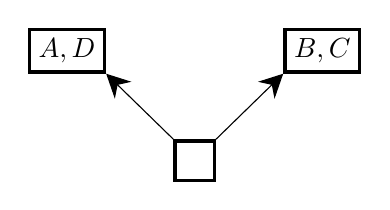
\begin{tikzpicture}[squarednode/.style={rectangle, draw, very thick, minimum size=5mm}]
			\node (center) {};
			\node[squarednode]      (right)   [right=of center] {$B, C$};
			\node[squarednode]      (left)    [left=of center] {$A, D$};
			\node[squarednode]      (lower)       	[below=of center] {};
			\draw[-{Stealth[length=3mm, width=3mm]}] (lower.north west) -- (left.south east);
			\draw[-{Stealth[length=3mm, width=3mm]}] (lower.north east) -- (right.south west);			
		\end{tikzpicture}
	\end{center}
	\vspace*{-.3cm}where at each node the true propositions are indicated.\pagebreak
	
	There is a corresponding classical counter-model $\mathcal M = (M, I)$ to $\varphi^\circ$ with $M = \{u, u_l, u_r\}$, $A^{I}(l) = D^I(l) = B^I(r) = C^I(r) = 1$ and $0$ else.
	
	Denoting $\psi_1 := (A\to B)\to C$ and $\psi_2 := (A\to B)\to C$ this corresponds to a counter-model $\mathcal M_T = (M_T, I_T)$ of $\varphi^\circ$ with $M_T = \{\epsilon, \psi_1, \psi_2, \psi_1\psi_2, \psi_2\psi_1\}$ and interpretation as presented below
	\begin{center}
		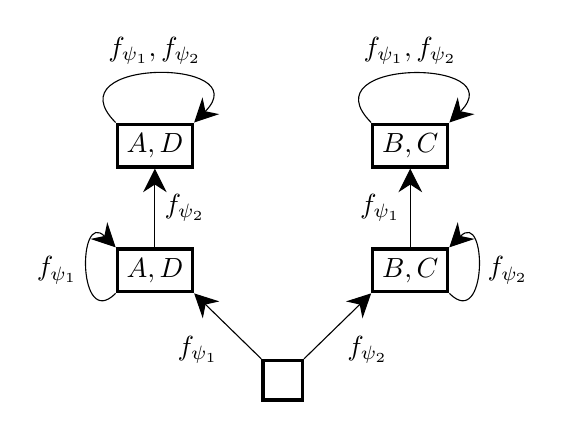
\begin{tikzpicture}[squarednode/.style={rectangle, draw, very thick, minimum size=5mm}]
			\node (center) {};
			\node[squarednode]      (right1)   [right=of center] {$B, C$};
			\node[squarednode]      (right2)   [above=of right1] {$B, C$};
			\node[squarednode]      (left1)    [left=of center] {$A, D$};
			\node[squarednode]      (left2)    [above=of left1] {$A, D$};
			\node[squarednode]      (lower)       	[below=of center] {};
			\draw[-{Stealth[length=3mm, width=3mm]}] (lower.north west) -- (left1.south east) node [midway, below left] {$f_{\psi_1}$};
			\draw[-{Stealth[length=3mm, width=3mm]}] (lower.north east) -- (right1.south west) node [midway, below right] {$f_{\psi_2}$};
			\draw[-{Stealth[length=3mm, width=3mm]}] (left1.north) -- (left2.south) node [midway, right] {$f_{\psi_2}$};
			\draw[-{Stealth[length=3mm, width=3mm]}] (right1.north) -- (right2.south) node [midway, left] {$f_{\psi_1}$};
			\draw[-{Stealth[length=3mm, width=3mm]}] (left1.south west) to [out=225, in=135, loop, looseness=3] node [left] {$f_{\psi_1}$} (left1.north west);		
			\draw[-{Stealth[length=3mm, width=3mm]}] (right1.south east) to [out=315, in=45, loop, looseness=3] node [right] {$f_{\psi_2}$} (right1.north east);
			\draw[-{Stealth[length=3mm, width=3mm]}] (left2.north west) to [out=135, in=45, loop, looseness=3] node [midway, above] {$f_{\psi_1}, f_{\psi_2}$} (left2.north east);
			\draw[-{Stealth[length=3mm, width=3mm]}] (right2.north west) to [out=135, in=45, loop, looseness=3] node [midway, above] {$f_{\psi_1}, f_{\psi_2}$} (right2.north east);		
		\end{tikzpicture}
	\end{center}
\end{example}

So we know that $\varphi^\circ$ is valid iff it is valid for structures that have as a domain the sequences without repetition over $\mathcal F_\to$, ordered by the prefix-relation and $$s^I = \epsilon, f_\psi^I(x) = \begin{cases}
	x&\text{ if $\psi$ occurs in $x$}\\
	x\psi&\text{ otherwise}
\end{cases}$$ Now we can replace all $\forall$-quantifiers by enumerating all the ground terms and finally all distinct ground instances of relations by new propositional variables yielding a CPC formula. This gives us the following translation:

\begin{definition}
	Suppose $\mathcal S$ is a set of formulas $\psi$ of the form
	$$A_\psi\to (B_\psi\wedge C_\psi), (A_\psi\wedge B_\psi)\to C_\psi, A_\psi\to (B_\psi\vee C_\psi),(A_\psi\vee B_\psi)\to C_\psi, (A_\psi\to B_\psi)\to C_\psi$$
	Let $\mathcal F_\to$ be the set of formulas of the form $(A\to B)\to C$ and $\Lambda$ the set of sequences without repetition over $\mathcal F_\to$. For each atom $A$ occurring in $\mathcal S$ and $k\in \mathcal F_\to$ consider a new atom $A^{k}$, which will correspond to $A^{I_F}(k)$ from the previous definition. Obtain $\mathcal S^\#$ by including the formulas
	\begin{itemize}
		\item $A^k\to A^{k\psi}$ for each $A$ occurring in $\mathcal S$, $k\in\Lambda$ and $\psi\in\mathcal F_\to$ not occurring in $k$.
		\item $A^k_\psi\to (B^k_\psi\circ C^k_\psi)$ for each $\circ\in\{\wedge,\vee\}$, $A_\psi\to (B_\psi\circ C_\psi)\in\mathcal S$, $k\in\Lambda$.
		\item $(A^k_\psi\circ B^k_\psi)\to C^k_\psi$ for each $\circ\in\{\wedge,\vee\}$, $A_\psi\to (B_\psi\circ C_\psi)\in\mathcal S$, $k\in\Lambda$.
		\item $(A^{k\psi}_\psi\to B^{k\psi}_\psi)\to C^k_\psi$ for $(A_\psi\to B_\psi)\to C_\psi\in\mathcal S$, $k\in\Lambda$ if $\psi$ does not occurr in $k$.
	\end{itemize}
\end{definition}

\begin{theorem}
	$$\mathcal S\models_C P\text{ iff }\mathcal S^\#\models_I P^\emptyset$$
\end{theorem}

\begin{example}
	Let us consider the law of excluded middle $\varphi = A\vee\neg A$. Then we get
	$$\mathcal S^-(\varphi) = \{(P_A\vee P_{\neg A})\to P_\varphi, A\to P_A, (A\to \bot)\to P_{\neg A}\}$$
	and we know that $\varphi$ is valid iff $\bigwedge \mathcal S(\varphi)\to P_\varphi$ is valid. Applying the above lemma this is intuitionistically valid iff $\bigwedge\mathcal S^\#\to P^\emptyset_\varphi$ is classically where, setting $\psi = (A\to \bot)\to P_{\neg A}$,
	\begin{align*}
		\mathcal S^\# =&\{P_\varphi^\epsilon\to P_\varphi^{\psi}, P_A^\epsilon\to P_A^{\psi},P_{\neg A}^\epsilon\to P_{\neg A}^{\psi},A^\epsilon\to A^{\psi}\}\\ &\cup\{(P_A^\epsilon\vee P_{\neg A}^\epsilon)\to P_\varphi^\epsilon, (P_A^{\psi}\vee P_{\neg A}^{\psi})\to P_\varphi^{\psi},  A^\epsilon\to P_A^\epsilon\}\\ &\cup \{P_A^{\psi}\to P_A^{\psi}, (A^{\psi}\to \bot)\to P_{\neg A}^\epsilon, (A^{\psi}\to \bot)\to P_{\neg A}^{\psi}\}
	\end{align*}
	It is easy to construct a counter example:
	$$P_\varphi^\epsilon  = P_A^\epsilon = P_{\neg A}^\epsilon = A^\epsilon = 0$$
	$$P_{\varphi}^{\psi} = P_A^{\psi} =  P_{\neg A}^{\psi} = A^{\psi} = 1$$
\end{example}	

\section{IPC to QBF}

It is well known that a polynomial time translation between QBF and IPC must exists, since both problems are PSPACE complete~\cite{garey1979computers, statman1979intuitionistic}. However giving an explicit translation from IPC to QBF can still be useful as good solvers exists for QBF but for IPC not so much. The translation from the last section will serve as a useful tool for this. We will not explain the semantics of QBF in depth. Intuitively just think that the interpretation of existentially quantified variables may depend on variables quantified above them.

Fix some set $\mathcal S$ of formulas $\psi$ of the form $$A_\psi\to (B_\psi\wedge C_\psi), (A_\psi\wedge B_\psi)\to C_\psi, A_\psi\to (B_\psi\vee C_\psi), (A_\psi\vee B_\psi)\to C_\psi, (A_\psi\to B_\psi)\to C_\psi$$and$$\varphi = \bigwedge \mathcal S\to P$$
and denote with $\mathcal F_\to$ the set of formulas of the form $(A\to B)\to C$. We will now formulate a QBF that expresses that $\varphi$ has an intuitionistic counter-model. The idea how to get a linear-size formula is: Instead of expressing validity at every node of $\mathcal M_T$ - which was done in the CPC translation - we express that on each path in $\mathcal M_T$ the nodes satisfy all conditions for $\mathcal M_T$ being a counter-model. The universally quantified variables $F_\psi$ in the next definition handle the branching, i.e. express which path is considered.

\begin{definition}
	For every propositional variable $X$ occurring in $\mathcal S$ and non-negative integer $n$ consider a new atom $X^n$ and for every formula $\psi\in\mathcal F_\to$ consider a new atom $F_\psi^n$. Let $\vec X^n$ range over all propositional variables $X^n$ and $\vec F^n$ range over all $F_\psi^n$. Define
	\begin{itemize}
		\item {\normalfont Valid}$(n)$ which encodes that $\vec F^n_\psi$ represents a valid next element of a sequence without repetition, i.e. if we interpret the $\vec F^i$ as bit-vectors, then $\vec F^n$ has exactly one bit set to $1$, indicating the formula at the $n$-th position of the sequence, and it is at a position that is $0$ in $\sum\{\vec F^i\:|\:i < n\}$.
		\item {\normalfont Persistent}$(n)$ which encodes that the persistency condition holds.
		\item {\normalfont Sat}$_{\mathcal S}(n)$ encoding that the formulas in $\mathcal S\setminus\mathcal F_\to$ hold at the $n$-th world of the path.
		\item {\normalfont Sat}$_{\mathcal F_\to}(n)$ encoding that the formula in $\mathcal F_\to$ that is represented by $\vec F^{n-1}$ holds.
	\end{itemize}
	Have $k = |\mathcal F_\to|$ and define$$\varphi^Q_{i} = \exists \vec X^i\forall \vec F^i\left(\text{\normalfont Persistent}(i)\wedge \text{\normalfont Sat}_{\mathcal S}(i)\wedge \text{\normalfont Sat}_{\mathcal F_\to}(i)\wedge\left(\text{\normalfont Valid}(i)\to \varphi^Q_{i+1}\right)\right)$$
	for $0 < i < k$ as well as the special cases
	$$\varphi^Q_{k} = \exists \vec X^k\left(\text{\normalfont Persistent}(k)\wedge \text{\normalfont Sat}_{\mathcal S}(k)\wedge \text{\normalfont Sat}_{\mathcal F_\to}(k)\right)$$
	for leafs and
	and $$\varphi^Q = \varphi_0^Q = \exists \vec X^0\forall \vec F^0\left(\neg P^0\wedge \text{\normalfont Sat}_{\mathcal S}(0)\wedge(\text{\normalfont Valid}(0)\to \varphi_1^Q)\right)$$for the root.
	Example encodings of the above formulas would be
	\begin{align*}
		\text{\normalfont Valid}(n) = &\left(\bigvee \{\mathcal F^n_\psi\:|\:\psi\in\mathcal F_\to\}\right)\wedge\left(\bigwedge \{\neg(F^n_{\psi_1}\wedge F^n_{\psi_1})\:|\:\psi_1\neq\psi_2\in\mathcal F_\to\}\right)\wedge\\&\wedge\left(\bigwedge\left\{\bigwedge\{F^i_\psi\to\neg F^n_\psi\:|\:i < n\}\:|\:\psi\in\mathcal F_\to\right\}\right)\\
		\text{\normalfont Persistent}(n) = & \bigwedge\{X^{n-1}\to X^n\:|\: X \text{ prop. variable with }X^{n-1}\in\vec X^{n-1}, X^n \in\vec X^{n}\}\\
		\text{\normalfont Sat}_{\mathcal S}(n) = &\bigwedge\left\{(A^n\circ B^n)\to C^n\:|\:(A\circ B)\to C\in \mathcal S\setminus\mathcal F_\to\right\}\wedge\\
		&\bigwedge\left\{A^n\to (B^n\circ C^n)\:|\:A\to (B\to C)\in \mathcal S\setminus\mathcal F_\to\right\}\\
		\text{\normalfont Sat}_{\mathcal F_\to}(n) = & \bigwedge\{F^{n-1}_\psi\to (A^n\to B^n)\to C^{n-1}\:|\:\psi = (A\to B)\to C\in\mathcal F_\to\}
	\end{align*}
\end{definition}

\begin{example}
	With the above encodings for double negation elimination $\varphi = ((A\to \bot)\to \bot)\to A$ we have
	$$\hspace*{-.3cm}
	\varphi^Q = \exists A^0\forall F^0\left(\neg A^0\wedge\left(F^0\to \exists A^1\left((A^0\to A^1)\wedge(F_0\to (A^1\to \bot)\to \bot)\right)\right)\right)
	$$
	which is a satisfiable QBF since $A^0 = 0, A^1 = 1$ satisfies it for any $F^0$.
\end{example}


\begin{lemma}
	$\varphi$ is not intuitionistically valid iff $\varphi^Q$ is a satisfiable QBF.
\end{lemma}
\begin{proof}
	Suppose $\varphi$ is not intuitionistically valid, i.e. there exists a counter-model $\mathcal M$ for $\mathcal S^\#\to P^\epsilon$. For each atom $A$ interpret $A^0$ such as $\mathcal M$ interprets $A^\epsilon$. Suppose we are given interpretations of all atoms $A^i$ for $i < n$ and a sequence with no repetitions $\psi_1\dots\psi_{n-1}$ over $\mathcal F_\to$ such that $\psi_i$ is exactly the $\psi\in\mathcal F_\to$ for which $F_{\psi}^i$ is true and $A^i$ is interpreted as $A^{\psi_1\dots\psi_i}$ is in $\mathcal M$.
	
	Let the $F^{n}_\psi$ be arbitrarily interpreted (since they are $\forall$-quantified). If not exactly one is interpreted as true then valid$(n)$ fails, i.e. have $\psi_n\in\mathcal F_\to$ the only element with $F^n_{\psi_n} = 1$. If $F^i_{\psi_n} = 1$ for some $i < n$ then valid$(n)$ also fails, so we may assume that $\psi_1\dots\psi_n$ is a sequence with no repetitions. Interpret the atoms $A^n$ as $\mathcal M$ interprets $A^{\psi_1\dots\psi_n}$. Continue this construction until $n  = |\mathcal F_\to|$. Then from $\mathcal M$ being a counter-example to $\mathcal S^\#\to P$ it directly follows that this interpretation satisfies $\varphi^Q$.
	
	On the other hand suppose $\varphi^Q$ is satisfiable. We construct a counter-example to $\varphi^\#$.
	Again we proceed iteratively. Interpret $A^\epsilon$ such as $A^0$ is interpreted in some satisfying interpretation of $\varphi^Q$. Suppose we are given a sequence $\psi_1\dots \psi_{n-1}$ such that for $i<n$ having $A^i = A^{\psi_0\dots\psi_{n-1}}$ is part of a satisfying interpretation of $\varphi^Q$ in which $F^i_\psi$ is chosen true iff $\psi = \psi_i$. Let $\psi_n\in\mathcal F_\to$. Consider some interpretation of the $A^n$ that are part of a satisfying assignment where $F^n_\psi$ is true iff $\psi = \psi_n$ and all variables quantified above are chosen as before. Have $A^{\psi_0\dots\psi_n} = A^n$ for each propositional variable $A$. From the definitions it directly follows that construction yields a counter-model for $\varphi^\#$.
\end{proof}

Since we have not discussed QBF in detail the above argument might be a bit difficult to follow, in particular the second part, but is simple in essence. We shall demonstrate with help of a example.

\begin{example}
	Consider the formula $\varphi = (((A\to B)\to C)\wedge((B\to A)\to C))\to C$, which is a non-intuitionistic tautology. Its associated QBF is $$\varphi^Q = \exists A^0B^0C^0\forall F_{\psi_1}^1F_{\psi_2}^1 \exists A^1B^1C^1\forall F_{\psi_1}^2F_{\psi_2}^2 \exists A^2B^2C^2\psi'$$where $\psi_1 := (A\to B)\to C, \psi_2 = (B\to A)\to C$ and $$\psi' = \bigwedge\left\{\begin{matrix}
		F^1_{\psi_1}\vee F^1_{\psi_2}, \neg(F^1_{\psi_1}\wedge F^1_{\psi_2}), F^2_{\psi_1}\vee F^2_{\psi_2},\neg(F^2_{\psi_1}\wedge F^2_{\psi_2}),\\F^1_{\psi_1}\to\neg F^2_{\psi_1},F^1_{\psi_2}\to\neg F^2_{\psi_2}, A^0\to A^1,A^1\to A^2,
		\\B^0\to B^1, B^1\to B^2, C^0\to C^1, C^1\to C^2,\neg C^0, \\
		F^1_{\psi_1}\to (A^1\to B^1)\to C^0, F^1_{\psi_2}\to(B^1\to A^1)\to C^0\\
		F^2_{\psi_1}\to (A^2\to B^2)\to C^1, F^2_{\psi_2}\to(B^2\to A^2)\to C^1
	\end{matrix}\right\}$$
	This QBF is satisfiable: Have $P^0 = 0$ for all atoms $P$, always $P^2 = 1$ for all atoms $P$ and $C^1 = 1$. Furthermore have $A^1 = 1$ iff $F^1_{\psi_1} = 1$ and $B^1 = 1$ iff $F^1_{\psi_2} = 1$. The construction of an counter-model to $\varphi^\#$ then proceeds as follows:
	\begin{itemize}
		\item First have $P^\epsilon = 0$ for each propositional variable $P$.
		\item For $P^{\psi_1}$ we consider what happens when we choose $F^1_{\psi_1}$ to be true, i.e. we have $A^{\psi_1} = C^{\psi_1} = 1$ and $0$ for all other propositional variables.
		\item For $P^{\psi_2}$ we consider what happens when we choose $F^1_{\psi_2}$ to be true, i.e. we have $B^{\psi_1} = C^{\psi_1} = 1$ and $0$ for all other propositional variables.
		\item Finally for $P^{\psi_1\psi_2} = P^{\psi_2\psi_1} = 1$ for all propositional variables $P$ as $P^2$ is true regardless of choice for the $F^i_\psi$.
	\end{itemize}
\end{example}	

Note that the last set of existentially quantified variables is superfluous because there is only one assignment which even has the chance to falsify $\varphi^Q$, namely that which assigns $1$ to the only $F_\psi^n$ such that $F_\psi^i = 0$ for all $i < n$. That is in our final formula we can replace $F_\psi^n$ with $\bigwedge\{\neg F_\psi^i\:|\:i < n\}$ and remove that quantification over $F_\psi^i$. With that we get the following:

\begin{corollary}
	Let $N$-INTINVALID be the problem of deciding if a formula $\bigwedge \mathcal S\to P$ as above with $|\mathcal F_\to|\leq N$ is not intuitionistically valid. Then $N$-INTINVALID is in $\Sigma_{2N-1}^P$. The dual problem $N$-INTVALID is in $\Pi_{2N-1}^P$.
\end{corollary}

\section{CQC to IQC}

We now give an analogous transformation for first order logic. However our trick of lifting the sentence to first-order logic to encode the Kripke semantics no longer works in such a straightforward manner, since we already are in first-order logic. However we do it nonetheless! The domain of our classical model will feature on the one hand elements representing worlds in a Kripke frame and on the other hand the domain-elements from the Kripke model. We reconcile these notions by introducing a special binary predicate $E$, first considered in~\cite{baaz2006skolemization} and expanded onto in~\cite{iemhoff2010eskolemization}, where $E(x, u)$ encodes that $x$ is an element of the domain of the world $u$. We fix some signature $\Sigma$ for this section. To encode that some $n$-ary relation $A$ holds at a world $u$ we replace each $n$-ary relation symbol $A$ with a $n+1$-ary relation symbol $A^\#$, interpreting $A^\#(\vec x, u)$ as "$A(\vec x)$ holds at u". Furthermore we write $\vec E(\vec x, u)$ for $\bigwedge\{E(x_i, u)\:|\:x_i\in \vec x\}$. 

First of all recall that due to Lemma~\ref{equivalid} it is sufficient to consider sentences of the form $\bigwedge\mathcal S\to P$ where all formulas in $\mathcal S$ are of one of the forms

$$\forall \vec z(A(\vec a)\to (B(\vec b)\wedge C(\vec c))), \forall \vec z((A(\vec a)\wedge B(\vec b))\to C(\vec c)),$$$$ \forall \vec z(A(\vec a)\to (B(\vec b)\vee C(\vec c))),
\forall \vec z((A(\vec a)\vee B(\vec b))\to C(\vec c)),$$$$ \forall \vec z((A(\vec a)\to B(\vec b))\to C(\vec c)),\forall \vec z(\forall xA(\vec a)\to B(\vec b)),$$$$ \forall \vec z(A(\vec a)\to\forall xB(b)), \forall \vec z(\exists xA(\vec a)\to B(\vec b)), \forall \vec z(A(\vec a)\to\exists xB(b))$$	
As in the propositional case we will now encode the Kripke Semantics, this time not only the relation $\preceq$ but also $E$ has to be axiomatized. For that we use the following predicates:
\begin{itemize}
	\item PartialOrder($\preceq$) encoding that $\preceq$ is a partial order.
	\item DomainSubset$(u, w)$ encoding that the domain at $u$ is a subset of that at $w$.
	\item World($u$) encoding that $u$ represents a world.
	\item DomainClosed($u$) which encodes that at $u$ the domain is closed under functions, e.g. contains all interpretations of constants.
	\item Persistent$(u, w)$ which encodes that persistency is satisfied between $u$ and $w$, i.e. for all predicates $A$ and domain elements $x$ with $A(x)$ at $u$ we have $A(x)$ at $w$.
\end{itemize}
Then analogously to the predicate case define
\begin{align*}
	K(\varphi) = \:& \text{PartialOrder}(\preceq) \wedge \\
				 & \forall u \forall w (u\preceq w\to \text{DomainSubset}(u, w)) \wedge\\
				 & \forall u(\text{World(u)}\to \text{DomainClosed}(u))\wedge\\
				 & \forall u\forall w (u\preceq w\to \text{Persistent}(u, w))
\end{align*}
Example encodings could be
\begin{align*}
	\text{PartialOrder}(\preceq) = &\:\forall u(u\preceq u)\wedge\forall u\forall w(u\preceq w\to w\preceq u\to u = w)\wedge\\&\:\forall u\forall v\forall w(u\preceq v\to v\preceq w\to u\preceq w)\\
	\text{DomainSubset}(u, w) = &\:\forall z(E(z, u)\to E(z, w))\\
	\text{World}(u) = &\:\exists xE(x, u)\\
	\text{DomainClosed}(u) = &\:\bigwedge\{\forall\vec z(\vec E(\vec z, u)\to E(f(\vec z), u))\:|\:\text{$f\in\Sigma$ is a function symbol}\}\\
	\text{Pesistent}(u, w) = &\:\bigwedge\{\forall\vec z(\vec A^\#(\vec z, u)\to A^\#(\vec z, w))\:|\:\text{$A\in\Sigma$ is a relation symbol}\}
\end{align*}

Using $E$ we then obtain $\mathcal S^\circ$ analogously to the predicate case by including formulas:

\begin{itemize}
	\item $\forall \vec z\forall u(s\preceq u\to \vec E(\vec z, u)\to (A^\#(\vec a, u)\to (B^\#(\vec b, u)\circ C^\#(\vec c, u))))$\\for each $\circ\in\{\wedge, \vee\}, \psi = \forall \vec z(A(\vec a)\to (B(\vec b)\circ C(\vec c)))\in\mathcal S$
	\item $\forall \vec z\forall u(s\preceq u\to\vec E(\vec z, u)\to (A^\#(\vec a, u)\circ B^\#(\vec b, u))\to C^\#(\vec c, u))$\\for each $\circ\in\{\wedge, \vee\}, \psi = \forall \vec z((A(\vec a)\circ B(\vec b))\to C(\vec c))\in\mathcal S$
	\item $\forall \vec z\forall u(s\preceq u\to\vec E(\vec z, u)\to\forall w(u\preceq w\to A^\#(\vec a, w)\to B^\#(\vec b, w))\to C^\#(\vec c, u))$\\ for each $\psi = \forall \vec z((A(\vec a)\to B(\vec b))\to C(\vec c))\in\mathcal S$
	\item  $\forall \vec z\forall u(s\preceq u\to\vec E(\vec z, u)\to \forall w(u\preceq w\to \forall x(E(x, w)\to A^\#(\vec a, w)))\to B^\#(\vec b, u))$\\for each $\forall \vec z(\forall xA(\vec a)\to B(\vec t_B))\in\mathcal S$.
	\item $\forall \vec z\forall u(s\preceq u\to\vec E(\vec z, u)\to A^\#(\vec a, u)\to \forall x(E(x, u)\to B^\#(\vec b, u)))$\\for each $\forall \vec t(A(\vec a)\to \forall xB(\vec b))\in\mathcal S$.
	\item $\forall \vec z\forall u(s\preceq u\to\vec E(\vec z, u)\to \exists x(E(x, u)\wedge A^\#(\vec z, u))\to B^\#(\vec b))$\\for each $\forall \vec z(\exists xA(\vec a)\to B(\vec b))\in\mathcal S$
	\item $\forall \vec z\forall u(s\preceq u\to\vec E(\vec z, u)\to A^\#(\vec b)\to \exists x(E(x, u)\wedge B^\#(\vec b, u)))$\\for each $\forall \vec z(A(\vec a)\to \exists xB(\vec b))\in\mathcal S$
\end{itemize}

Then $\varphi = \bigwedge\mathcal S\to P$ is intuitionistically valid iff
$$\varphi^\circ= \text{World}(s)\to K(\varphi)\to \bigwedge S^\circ\to P^\#(s)$$
is classically valid where $s$ is a new constant symbol. This was obvious in the propositional case but here it is more nuanced, so let's present a proof.

\begin{proof}
	We proceed by translation of counter-examples. Suppose first we have a counter-example $\mathcal M = (M, I)$ to $\varphi^\circ$. As a Kripke frame $(W, \leq)$ take all $ W = \{m\in M\:|\:\text{ World}^I(m)\}$ let $\leq$ be $\preceq^I$ restricted to $W$. Then let $M_u = \{m\in M\:|\: E(m, u)\}$ and let $f^{I_u}$ be $f^I$ restricted to $M_u$ and $A^{I_u}(\vec x): \Leftrightarrow A^\#(\vec x, u)$. It is then a straightforward check of definitions that this defines a Kripke counter-model to $\varphi$.
	
	The other direction is a bit more involved. Suppose we have a Kripke counter-model to $\varphi$ with Frame $(W, \preceq)$ and family of $\Sigma$-structures $(M_w, I_w)_{w\in W}$. In particular since it is a counter-model there exists $w_0\in W$ with $w_0\not\models\varphi$. Let $W_0 = \{w\in W\:|\: w\geq w_0\}$ and define an equivalence relation $\sim$ on $\{(x, u)\:|\:u\in W_0, x\in M_u\}$ via $(x, u)\sim (y, w)$ iff $x = y$ and there exists $v\in W_0$ comparable with both $u, w$ such that $x\in v$ and denote the equivalence class of $(x, u)$ with $[x, u]$. Let $M = W_0\cup \{[x, u]\:|\:u\in W_0, x\in M_u\}$ and extend $\sim$ by having $[w] = \{w\}$ for $w\in W_0$. Now have
	\begin{itemize}
		\item $s^I = w_0$.
		\item $E^I(m, w)$ iff $w\in W_0$ and $m \sim [x, w]$ for some $x\in M_w$.
		\item $f^I(m_1\dots m_n) =\begin{cases}
			 f^{I_u}(x_1\dots x_n) &\text{if there are $ u\in W_0, x_i\in M_u$ with $m_i\sim [x_i, u]$ for all $i$}\\
			 w_0 & \text{otherwise}
		\end{cases}$
		\item ${A^\#}^I(m_1\dots m_n, u) \Leftrightarrow\begin{cases}
			A^{I_u}(x_1\dots x_n) &\text{if $u\in W_0$ and $\exists x_i\in M_u$ w. $m_i\sim [x_i, u]$ for all $i$}\\
			\top & \text{otherwise}
		\end{cases}$
	\end{itemize}
	One easily verifies that these are well-defined. Let us now briefly check that this indeed defines a counter-model. First of all ${P^\#}^I(s^I)$ is false since $P^{I_{w_0}}$ is. Clearly World$(w_0)$ holds and $K(\varphi)$ is also easily verified. All that remains to show is $M, I\models\bigwedge\mathcal S^\circ$. Consider e.g. the case where $\psi\in\mathcal S$ is of the form
	$$ \forall \vec z((A(\vec a)\to B(\vec b))\to C(\vec c))$$
	We have to show that
	$$M, I\models \forall \vec z\forall u(\vec E(t, u)\to \forall w(u\preceq w\to A^\#(\vec a, w)\to B^\#(\vec b, w))\to C^\#(\vec c, u))$$
	holds. Suppose towards contradiction that it does not, i.e. there are $u, \vec z\in M$ such that for all $w\in M$
	$$\vec E^I(\vec z, u)\to (u\preceq w\to {A^\#}^I(\vec a, w)\to {B^\#}^I(\vec b, w))\to {C^\#}^I(\vec c, u)$$ is false. For that ${C^\#}^I(\vec c, u)$ must be false and in particular $u\in W_0$. Futhermore $\vec E^I(\vec z, u)$ must be true and we can write $\vec z = [z_1, u]\dots[z_n, u]$ for some $z_i\in W_u$. Note that the above is false in particular for $w\in M_0$ with $u\preceq w$. But this would imply
	$$((A^{I_u}(\vec a)\to B^{I_u}(\vec b))\to C^{I_u}(\vec c))[\vec z/z_1\dots z_n]$$in our original Kripke counter-model. The other cases are analogous.
\end{proof}

We proceed now as in the previous section. Denote the set of formulas $\psi\in\mathcal S$ of the form $\forall\vec z((A(\vec a)\to B(\vec b))\to C(\vec c))$ with $\mathcal F_\to$ and of the form $\forall \vec z(\forall xA(\vec a)\to B(\vec b))$ with $\mathcal F_\forall$. Let $\mathcal F = \mathcal F_\to\cup\mathcal F_\forall$. For each  $\psi\in\mathcal F$ consider a new function symbol $f$. As before we may assume that $s$ is a least element and eliminate the quantification over $w$ by replacing formulas
$$\forall \vec z\forall u(s\preceq u\to\vec E(\vec z, u)\to \forall w(u\preceq w\to A^\#(\vec a, w)\to B^\#(\vec b, w))\to C^\#(\vec c, u))$$ with
$$\forall \vec z\forall u(\vec E(\vec z, u)\to (A^\#(\vec a, f(\vec z, u))\to B^\#(\vec b, f(\vec z, u)))\to C^\#(\vec c, u))$$ and
$$\forall \vec z\forall u(s\preceq u\to\vec E(\vec z, u)\to \forall w(u\preceq w\to \forall x(E(x, w)\to A^\#(\vec a, w)))\to B^\#(\vec b, u))$$ with $$\forall \vec z\forall u(\vec E(\vec z, u)\to (\forall x(E(x, f(\vec z, u))\to A^\#(\vec a, f(\vec z, u))))\to B^\#(\vec b, u))$$
and in each other formula in $\mathcal S^\circ$ remove the $s\preceq u$ to obtain $\mathcal S^\#$ from $\mathcal S^\circ$. Then the previous formulas are equivalid to
$$\varphi^\circ= \forall u(s\preceq u)\to \bigwedge\{\forall \vec t\forall u(u\preceq f(\vec z, u))\:|\:\psi\in\mathcal F\}\to K(\varphi)\to\bigwedge\mathcal S^\#\to P^\#$$
As in the previous section we can define a tree-counter model for this.
\begin{definition}
	Suppose we are given a counter-model $\mathcal M = (M, I)$ for $\varphi^\circ$. For $\psi = \forall\vec t\psi'\in\mathcal F_\to$ we say that is it \textit{fulfilled} at $u\in M$ with $\vec a\in M^n$ iff $(A_\psi^I(\vec t_A, u)\to B_\psi^I(\vec t_B, u))[\vec a/\vec t]$ is false or $C_\psi^I(\vec t_C, u)[\vec a/\vec t]$ is true.
	For $\psi = \forall\vec t\psi'\in\mathcal F_\forall$ we say that it is \textit{fulfilled} at $u\in M$ with $\vec a\in M^n$ iff there is $a\in M_u$ such that $A^{I[a/x]}_\psi(\vec t_A)[\vec a/\vec t]$ is false or $B_\psi^I(\vec t_B)[\vec a/\vec t]$ is true. For $\psi\in\mathcal F$ define $$g_{\vec a, \psi} : M\to M, u\mapsto\begin{cases}
		u&\text{ if $\psi$ is fulfilled in $u$ with $\vec a$}\\
		f^I_\psi(\vec a, u)&\text{ else}		
	\end{cases}$$		
	Define a $\mathcal M_T = (M_T, I_T)$ as follows:
	\begin{itemize}
		\item $M_T$ are the sequences on $\{ \vec t, \psi\:|\:\psi\in \mathcal F, \vec t\in M^n\}$ without repetition of elements $\vec t,\psi$ with $\psi\in\mathcal F_\to$ and without immediate repetition of elements $\vec t,\psi$ with $\psi\in\mathcal F_\forall$.
		\item Interpret $\preceq$ as the prefix-order.
		\item Have $$f_\psi^{I_T}(x_1\dots x_n) = \begin{cases}
			x_1\dots x_n&\text{if $x=x_n$}\\
			x_1\dots x_nx&\text{else}			
		\end{cases}$$
		\item For propositional variables $P$ have $$P^{I_T}(x_1\dots x_n) = P^I(g_{x_n}(\dots(g_{x_1}(s^I))\dots))$$
	\end{itemize}
\end{definition}

\begin{lemma}
	Let $\mathcal M = (M, I)$ be a counter-model to $\mathcal \varphi^\circ$.
	\begin{enumerate}
		\item $\psi$ is fulfilled at $f_\psi^I(\vec a, u)$ with $\vec a$ for all $u\in M, \psi\in\mathcal F$, $\vec a\in M^n$.
		\item If $\psi\in\mathcal F_\to$ is fulfilled at $u\in M$ with $\vec a$ then $\psi$ is fulfilled at all $w\geq u$ with $\vec a$.
	\end{enumerate}	
\end{lemma}

\begin{proof}
	For $\psi\in\mathcal F_\to$ the proof is analogous to the previous section.
	
	1. Let $\psi\in\mathcal F_\forall$. If $B^I_\psi(\vec b, u)[\vec a/\vec t]$ holds then we are done due to persistency. Otherwise there is $a$ with $E^I(a, f^I_\psi(\vec a, u))$ such that $A^{I[a/x]}_\psi(\vec t_A, f^I_\psi(\vec a, u))$ is false. So $\psi$ is fulfilled at $f^I_\psi(\vec a, u)$ with $\vec a$.
\end{proof}

Part 2 of this Lemma does not hold for $\psi\in\mathcal F_\forall$, because even if for all $x$ with $E(x, v$) we have $A(x, v)$ there could be some term $t$ with $\neg E(t, v)$ and $w$ with $v\preceq w$ such that $E(t, w)$ and $\neg A(t, w)$. This is why we must consider sequences that have repetitions of such formulas:

\begin{example}
	Consider the $\varphi = \neg(\neg \forall xA(x)\vee\neg \forall xB(x))$. There is a counter-model
	\begin{center}
		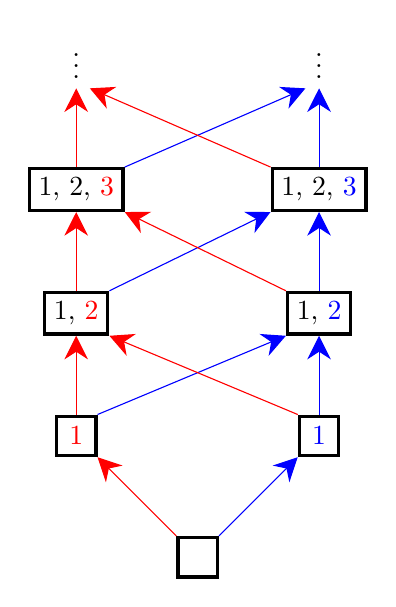
\begin{tikzpicture}[squarednode/.style={rectangle, draw, very thick, minimum size=5mm}]
			\node[squarednode]      (0)   [] {$ $};
			\node[squarednode]      (1r)   [above right=of 0] {{\color{blue}$1$}};
			\node[squarednode]      (1l)   [above left=of 0] {{\color{red}$1$}};
			\node[squarednode]      (2r)   [above=of 1r] {{1, \color{blue}$2$}};
			\node[squarednode]      (2l)   [above=of 1l] {{1, \color{red}$2$}};
			\node[squarednode]      (3r)   [above=of 2r] {{1, 2, \color{blue}$3$}};
			\node[squarednode]      (3l)   [above=of 2l] {{1, 2, \color{red}$3$}};
			\node      (4r)   [above=of 3r] {{$\vdots$}};
			\node      (4l)   [above=of 3l] {{$\vdots$}};
			\draw[-{Stealth[length=3mm, width=3mm]}, color=blue] (0.north east) -- (1r.south west);
			\draw[-{Stealth[length=3mm, width=3mm]}, color=red] (0.north west) -- (1l.south east);
			\draw[-{Stealth[length=3mm, width=3mm]}, color=blue] (1r.north) -- (2r.south);
			\draw[-{Stealth[length=3mm, width=3mm]}, color=red] (1l.north) -- (2l.south);
			\draw[-{Stealth[length=3mm, width=3mm]}, color=blue] (1l.north east) -- (2r.south west);
			\draw[-{Stealth[length=3mm, width=3mm]}, color=red] (1r.north west) -- (2l.south east);
			\draw[-{Stealth[length=3mm, width=3mm]}, color=blue] (2r.north) -- (3r.south);
			\draw[-{Stealth[length=3mm, width=3mm]}, color=red] (2l.north) -- (3l.south);
			\draw[-{Stealth[length=3mm, width=3mm]}, color=blue] (2l.north east) -- (3r.south west);
			\draw[-{Stealth[length=3mm, width=3mm]}, color=red] (2r.north west) -- (3l.south east);
			\draw[-{Stealth[length=3mm, width=3mm]}, color=blue] (3r.north) -- (4r.south);
			\draw[-{Stealth[length=3mm, width=3mm]}, color=red] (3l.north) -- (4l.south);
			\draw[-{Stealth[length=3mm, width=3mm]}, color=blue] (3l.north east) -- (4r.south west);
			\draw[-{Stealth[length=3mm, width=3mm]}, color=red] (3r.north west) -- (4l.south east);
		\end{tikzpicture}
	\end{center}
	where at each node the elements that exist at it are indicated. For black ones both $A$ and $B$ hold, for red ones only $B$, for blue ones only $A$. Furthermore red arrows indicate $f_{\neg \forall xA(x)}$ and blue arrows $f_{\neg \forall xB(x)}$. Note that applying $f_{\neg \forall xA(x)}$ we must always reach the left column and $f_{\neg \forall xB(x)}$ we must always reach the right column. Therefore applying $f_{\neg \forall xA(x)}\circ f_{\neg \forall xB(x)}$ we can never remain stationary. This is in contrast to the propositional case.
\end{example}


\begin{corollary}
	If $\mathcal M$ is a counter-model to $\varphi^\circ$ then so is $\mathcal M_T$.
\end{corollary}

Even if we don't have the nice finiteness of the propositional case we have still reduced the model complexity in that we know that considering worlds of the form $$f_{\psi_1}(\vec t_1, f_{\psi_2}(\vec t_2, \dots f_{\psi_n}(\vec t_n, s)\dots))$$ is sufficient. In particular this allows us to completely eliminate $\preceq$ from the formula, that is we remove the PO-encoding from $K(\varphi)$ and replace $\forall u\forall w\forall x((E(x, u)\wedge u\preceq w)\to E(x, w))$ with $\bigwedge\{\forall \vec z\forall u(E(x, u)\to E(x, f_\psi(\vec z, u)))\:|\:\psi\in\mathcal F_\to\}$ and analogously for persistency to obtain $K$. Define

$$\varphi^{\#} = K\to \bigwedge S^\#\to P^\#$$
then we have 
\begin{theorem}
	$\varphi$ is intuitionistically valid iff $\varphi^\#$ is classically valid.
\end{theorem}
The complete translation is summarised in Theorem~\ref{fullFOtranslation}.

\begin{example}
	Consider the double negation shift (DNS)
	$$\varphi = \forall x\neg\neg A(x)\to \neg\neg\forall x A(x)$$
	which is a famous non-intuitionistic tautology. We get
	\begin{align*}
		\mathcal S = & \{(P_{\forall x\neg\neg A(x)}\to P_{\neg\neg\forall xA(x)})\to P_\varphi, P_{\forall x\neg\neg A(x)}\to \forall xP_{\neg\neg A(x)}(x)\}\cup\\
		& \{\forall t((P_{\neg\neg A(x)}(t)\wedge P_{\neg A(x)}(t))\to \bot), \forall t((A(t)\to \bot)\to P_{\neg A(x)})(t)\}\cup\\
		& \{(P_{\neg\forall xA(x)}\to \bot)\to P_{\neg\neg\forall xA(x)}, (P_{\neg\forall xA(x)}\wedge P_{\forall xA(x)})\to \bot\}\cup\\
		&\{\forall xA(x)\to P_{\forall xA(x)}\}
	\end{align*}
	and thus, denoting $\psi_1 = (P_{\neg\forall xA(x)}\to \bot)\to P_{\neg\neg\forall xA(x)}$ and $\psi_2 = \forall xA(x)\to P_{\forall xA(x)}$, we have
	\begin{align*}
		\mathcal S^\# = & \{\forall u(P_{\forall x\neg\neg A(x)}(u)\to P_{\neg\neg\forall xA(x)}(u))\to P_\varphi(u)\}\cup\\& \{\forall u(P_{\forall x\neg\neg A(x)}(u)\to \forall xP_{\neg\neg A(x)}(x, u)\}\cup\\
		& \{\forall t, u((P_{\neg\neg A(x)}(t, u)\wedge P_{\neg A(x)}(t, u))\to \bot)\}\\& \{\forall t, u((A(t, u)\to \bot)\to P_{\neg A(x)}(t, u))\}\cup\\
		& \{\forall u((P_{\neg\forall xA(x)}(f_{\psi_1}(u))\to \bot)\to P_{\neg\neg\forall xA(x)}(u))\}\\& \{\forall u((P_{\neg\forall xA(x)}(u)\wedge P_{\forall xA(x)}(u))\to \bot)\}\cup\\
		&\{\forall u(\forall xA(x, f_{\psi_2}(u))\to P_{\forall xA(x)}(u))\}
	\end{align*}
\end{example}

\section{Conclusion}

We have presented a complete embedding of intuitionistic into classical logic. The transformation saw an exponential blow-up parametrized by $|\mathcal F_\to|$ in the propositional case and a complexity increase reflected by arity-increase of all relations and introduction of new function symbols in the predicate case. A key motivation for our work is the possibility of leveraging classical provers for showing intuitionistic validity. The practical feasibility of our translation is yet to be tested. In particular in the first-order case it is difficult to estimate how the increased complexity of the output formula impacts proof search. Initial tests show promise but we plan on conducting a more thorough evaluation. A key factor that is not yet clear is how large the parameters $|\mathcal F_\to|$ in the propositional case and $|\mathcal F|$ in the predicate case respectively are in practice.

The complexity increase fell directly out of our very straightforward construction. We plan to establish better bounds in future work by more intelligently utilizing structural properties of the formula, in particular by using that certain atoms are independent from each other it is possible to construct a smaller counter-example $\mathcal M_T$ in many cases. Besides improving the practical feasibility of our approach we hope that this will allow us to also give a new translation from QBF to IPC respecting complexity considerations and shine more light on the link between intuitionistic logic and the polynomial hierarchy.

We hope that this work will provide a foundation for a new practical approach to automated reasoning for intuitionistic logic, a problem that has not seen much progress in recent times.


\bibliography{lipics-v2021-EIICL}

\appendix

\section{Omitted Proofs}

\begin{lemma}\label{ap1}
	Let $\chi$ be a formula and $\{t_1\dots t_n\} = T$ contain all free variables in $\chi$, then for every structure $\mathcal M = (M, I)$ there exists $\mathcal M_\chi = (M, I_\chi$) such that $p^{I_{\chi}} = p^I$ for all function and relation symbols $p$ occurring in $\chi$ and for all variable assignments $v$ we have
	\begin{itemize}
		\item if $\mathcal M, v\models\chi$ then $\mathcal M_\chi, v\models\chi^S_T$.
		\item if $\mathcal M, v\not\models\chi$ then $\mathcal M_\chi, v\not\models\chi^H_T$.
	\end{itemize}
\end{lemma}

\begin{proof}
	We proceed by simultaneous induction on the formula height.
	
	For atomic $\chi$ the claims are clear.
	
	Otherwise there are $3$ cases:
	
	1. $\chi = \varphi\circ\psi$ for $\circ\in\{\wedge,\vee,\to\}$. By induction hypothesis there exist $\mathcal M_{\varphi, v} = (M, I_{\varphi, v}), \mathcal M_{\psi, v} = (M, I_{\psi, v})$ for $\varphi,\psi$ as in the lemma. Then we can define $I_{\chi, v}$ as follows:
	
	For every symbol $p$ that occurs in $\varphi^S$ or $\varphi^H$ but not $\psi^S, \psi^H$ have $p^{I_{\chi, v}} = p^{I_{\varphi, v}}$. For every symbol $p$ that occurs in $\psi^S$ or $\psi^H$ but not $\varphi^S, \varphi^H$ have $p^{I_{\chi, v}} = p^{I_{\psi, v}}$. Otherwise $p$ already occurs in $\varphi$ so have $p^{I_{\chi, v}} = p^I$.
	
	Let $\circ=\to$. Suppose $\mathcal M, v\models\chi$. Then $\mathcal M, v\not\models\varphi$ or $\mathcal M\models\psi$ and therefore $\mathcal M_\chi\not\models\varphi^S_T$ or $\mathcal M_\chi\models\psi^H_T$, i.e. $\mathcal M_\chi\models\chi^S_T$. On the other hand suppose $\mathcal M, v\not\models\chi$. Then $\mathcal M, v\models\varphi$ and $\mathcal M, v\not\models\psi$ and therefore $\mathcal M_\chi, v\models \varphi^S_T$ and $\mathcal M_\chi, v\not\models\psi^S_T$, i.e. $\mathcal M_\chi\not\models\chi^H_T$. Analogous arguments work for $\circ\in\{\wedge, \vee\}$.
	
	2. $\chi = \forall x\varphi$. Choose $s^{I_\chi}:M^n\to M$ such that $s^{I_\chi}(x_1,\dots, x_n) = m$ if there exists $m\in M$ such that $\mathcal M, v[x_1/t_1\dots x_n/t_n, m/a]\not\models\varphi[a/x]$ for all $v$ and arbitrary otherwise. Since $T$ contains all free variables occurring in $\chi$ this is a well-defined function.
	
	By induction hypothesis there exists a structure $\mathcal M_{\varphi[a/x]}$ as is the Lemma. Let $p^{I_\chi} = p^{I_{\varphi[a/x]}}$ for all symbols occurring in $\chi$ and $$p^{I_\chi}(x_1\dots x_{i-1}, x_{i+1}\dots x_m) = p^{I_{\varphi[a/x]}}(x_1\dots x_{i-1}, s^{I_\chi}(x_1\dots x_n), x_{i+1}\dots x_m)$$ for all symbols $p$ occurring in $\varphi[a/x]^S_{T\cup a}$ or $\varphi[a/x]^H_{T\cup a}$ but not in $\chi$ where $x_i$ is the argument corresponding to the free variable $a$.
	
	Suppose $\mathcal M, v\models\chi$. Then for all $m\in M$ $\mathcal M, v[m/a]\models\varphi[a/x]$ and therefore $\mathcal M_{\chi}, v[m/a]\models\varphi[a/x]^S_{M\cup\{a\}}$ and thus $\mathcal M_{\chi}, v\models \forall x\varphi([a/x]^S_{M\cup\{a\}}[x/a])$, i.e. $\mathcal M_\chi,v\models \chi^S$. On the other hand suppose $\mathcal M, v\not\models\chi$. Then there exists $m\in M$ such that $\mathcal M, v[m/a]\not\models\varphi[a/x]$ and therefore $\mathcal M_\chi, v[m/a]\not\models\varphi[a/x]^H_{T\cup\{a\}}$ and so by definition $\mathcal M_\chi, v\not\models\varphi[s(t_1,\dots t_n)/x]^H_T$, i.e. $\mathcal M_\chi, v\not\models(\forall x\varphi)^H_T$.
	
	3. $\chi = \exists x\varphi$. The argument runs dually to 2. Choose $s^{I_\chi}:M^n\to M$ such that $s^{I_\chi}(x_1,\dots, x_n) = m$ if there exists $m\in M$ such that for all $v$ we have $\mathcal M, v[x_1/t_1\dots x_n/t_n, m/a]\models\varphi[a/x]$ and arbitrary otherwise. Since $T$ contains all free variables occurring in $\chi$ this is a well-defined function.
	
	By induction hypothesis there exists a structure $\mathcal M_{\varphi[a/x]}$ as is the Lemma. Let $p^{I_\chi} = p^{I_{\varphi[a/x]}}$ for all symbols occurring in $\chi$ and $$p^{I_\chi}(x_1\dots x_{i-1}, x_{i+1}\dots x_m) = p^{I_{\varphi[a/x]}}(x_1\dots x_{i-1}, s^{I_\chi}(x_1\dots x_n), x_{i+1}\dots x_m)$$ for all symbols $p$ occurring in $\varphi[a/x]^S_{T\cup a}$ or $\varphi[a/x]^H_{T\cup a}$ but not in $\chi$ where $x_i$ is the argument corresponding to the free variable $a$.
	
	Then as in 2 from $\mathcal M, v\models \chi$ follows $\mathcal M_\chi,v\models\chi^S_T$ and from $\mathcal M, v\not\models \chi$ follows $\mathcal M_\chi,v\not\models\chi^H_T$.
\end{proof}

\begin{lemma}\label{ap2}
	For every structure $\mathcal M$ and $\{t_1\dots t_n\} = T$ that contains all free variables in $\chi$ and variable assignment $v$
	\begin{itemize}
		\item if $\mathcal M, v\models\varphi^S_T$ then $\mathcal M, v\models \varphi$
		\item if $\mathcal M, v\not\models\varphi^H_T$ then $\mathcal M, v\not\models\varphi$.
	\end{itemize}
\end{lemma}

\begin{proof}
	Again we proceed by simultaneous induction on the formula height.
	
	For atoms the claims are clear. We distinguish 5 cases.
	
	1. $\chi = \varphi\to\psi$. Suppose $\mathcal M, v\models\chi^S_T$, i.e. $\mathcal M, v\not\models\varphi^H_T$ or $\mathcal M, v\models\psi^S_T$. By induction hypothesis $\mathcal M, v\not\models \varphi$ or $\mathcal M, v\models\psi$, i.e. $\mathcal M, v\models \chi$. On the other hand suppose $\mathcal M, v\not\models\chi^H_T$, i.e. $\mathcal M, v\models\varphi^S_T$ and $\mathcal M, v\not\models\varphi^H_T$. Again by induction hypothesis $\mathcal M,v\models\varphi$ and $\mathcal M, v\not\models \varphi$, so $\mathcal M, v\not\models\chi$.
	
	2. + 3. Conjunctions and Disjunctions are dealt with analogously.
	
	4. $\chi = \forall x\varphi$.  Suppose $\mathcal M, v\models\chi^S_T$, i.e. for all $m\in M$ we have $\mathcal M, v[m/a]\models \chi[a/x]^S_{T\cup\{a\}}$ and by induction hypothesis $\mathcal M, v[m/a]\models \chi[a/x]$. Then it follows that $\mathcal M, v\models\varphi$. On the other hand suppose $\mathcal M, v\not\models\chi^H_T$, i.e. there exists $m\in M$ such that $\mathcal M, v[m/a]\not\models\chi[a/x]^H_{T\cup \{a\}}$, then by induction hypothesis $\mathcal M, v[m/a]\not\models \chi[a/x]$, i.e. $\mathcal M, v\not\models\forall x\chi$.
	
	5. $\chi = \exists x\varphi$.  The argument runs dually to 4.
\end{proof}


\end{document}
